\documentclass[twoside]{book}

% Packages required by doxygen
\usepackage{fixltx2e}
\usepackage{calc}
\usepackage{doxygen}
\usepackage[export]{adjustbox} % also loads graphicx
\usepackage{graphicx}
\usepackage[utf8]{inputenc}
\usepackage{makeidx}
\usepackage{multicol}
\usepackage{multirow}
\PassOptionsToPackage{warn}{textcomp}
\usepackage{textcomp}
\usepackage[nointegrals]{wasysym}
\usepackage[table]{xcolor}

% Font selection
\usepackage[T1]{fontenc}
\usepackage[scaled=.90]{helvet}
\usepackage{courier}
\usepackage{amssymb}
\usepackage{sectsty}
\renewcommand{\familydefault}{\sfdefault}
\allsectionsfont{%
  \fontseries{bc}\selectfont%
  \color{darkgray}%
}
\renewcommand{\DoxyLabelFont}{%
  \fontseries{bc}\selectfont%
  \color{darkgray}%
}
\newcommand{\+}{\discretionary{\mbox{\scriptsize$\hookleftarrow$}}{}{}}

% Page & text layout
\usepackage{geometry}
\geometry{%
  a4paper,%
  top=2.5cm,%
  bottom=2.5cm,%
  left=2.5cm,%
  right=2.5cm%
}
\tolerance=750
\hfuzz=15pt
\hbadness=750
\setlength{\emergencystretch}{15pt}
\setlength{\parindent}{0cm}
\setlength{\parskip}{3ex plus 2ex minus 2ex}
\makeatletter
\renewcommand{\paragraph}{%
  \@startsection{paragraph}{4}{0ex}{-1.0ex}{1.0ex}{%
    \normalfont\normalsize\bfseries\SS@parafont%
  }%
}
\renewcommand{\subparagraph}{%
  \@startsection{subparagraph}{5}{0ex}{-1.0ex}{1.0ex}{%
    \normalfont\normalsize\bfseries\SS@subparafont%
  }%
}
\makeatother

% Headers & footers
\usepackage{fancyhdr}
\pagestyle{fancyplain}
\fancyhead[LE]{\fancyplain{}{\bfseries\thepage}}
\fancyhead[CE]{\fancyplain{}{}}
\fancyhead[RE]{\fancyplain{}{\bfseries\leftmark}}
\fancyhead[LO]{\fancyplain{}{\bfseries\rightmark}}
\fancyhead[CO]{\fancyplain{}{}}
\fancyhead[RO]{\fancyplain{}{\bfseries\thepage}}
\fancyfoot[LE]{\fancyplain{}{}}
\fancyfoot[CE]{\fancyplain{}{}}
\fancyfoot[RE]{\fancyplain{}{\bfseries\scriptsize Generated by Doxygen }}
\fancyfoot[LO]{\fancyplain{}{\bfseries\scriptsize Generated by Doxygen }}
\fancyfoot[CO]{\fancyplain{}{}}
\fancyfoot[RO]{\fancyplain{}{}}
\renewcommand{\footrulewidth}{0.4pt}
\renewcommand{\chaptermark}[1]{%
  \markboth{#1}{}%
}
\renewcommand{\sectionmark}[1]{%
  \markright{\thesection\ #1}%
}

% Indices & bibliography
\usepackage{natbib}
\usepackage[titles]{tocloft}
\setcounter{tocdepth}{3}
\setcounter{secnumdepth}{5}
\makeindex

% Hyperlinks (required, but should be loaded last)
\usepackage{ifpdf}
\ifpdf
  \usepackage[pdftex,pagebackref=true]{hyperref}
\else
  \usepackage[ps2pdf,pagebackref=true]{hyperref}
\fi
\hypersetup{%
  colorlinks=true,%
  linkcolor=blue,%
  citecolor=blue,%
  unicode%
}

% Custom commands
\newcommand{\clearemptydoublepage}{%
  \newpage{\pagestyle{empty}\cleardoublepage}%
}

\usepackage{caption}
\captionsetup{labelsep=space,justification=centering,font={bf},singlelinecheck=off,skip=4pt,position=top}

%===== C O N T E N T S =====

\begin{document}

% Titlepage & ToC
\hypersetup{pageanchor=false,
             bookmarksnumbered=true,
             pdfencoding=unicode
            }
\pagenumbering{roman}
\begin{titlepage}
\vspace*{7cm}
\begin{center}%
{\Large My Project }\\
\vspace*{1cm}
{\large Generated by Doxygen 1.8.11}\\
\end{center}
\end{titlepage}
\clearemptydoublepage
\tableofcontents
\clearemptydoublepage
\pagenumbering{arabic}
\hypersetup{pageanchor=true}

%--- Begin generated contents ---
\chapter{Gin\+Gin\+Money}
\label{md_README}
\hypertarget{md_README}{}
Le git des gens qui essayent de faire un color flood Première modification Ceci est un test webhook 
\chapter{Data Structure Index}
\section{Data Structures}
Here are the data structures with brief descriptions\+:\begin{DoxyCompactList}
\item\contentsline{section}{\hyperlink{struct_composante_connexe}{Composante\+Connexe} }{\pageref{struct_composante_connexe}}{}
\item\contentsline{section}{\hyperlink{structt__case}{t\+\_\+case} }{\pageref{structt__case}}{}
\item\contentsline{section}{\hyperlink{structt___liste_composante_connexe}{t\+\_\+\+Liste\+Composante\+Connexe} }{\pageref{structt___liste_composante_connexe}}{}
\end{DoxyCompactList}

\chapter{File Index}
\section{File List}
Here is a list of all files with brief descriptions\+:\begin{DoxyCompactList}
\item\contentsline{section}{\hyperlink{_composante_connexe_8c}{Composante\+Connexe.\+c} }{\pageref{_composante_connexe_8c}}{}
\item\contentsline{section}{\hyperlink{_composante_connexe_8h}{Composante\+Connexe.\+h} }{\pageref{_composante_connexe_8h}}{}
\item\contentsline{section}{\hyperlink{_grille_8c}{Grille.\+c} }{\pageref{_grille_8c}}{}
\item\contentsline{section}{\hyperlink{_grille_8h}{Grille.\+h} }{\pageref{_grille_8h}}{}
\item\contentsline{section}{\hyperlink{_liste_composante_connexe_8c}{Liste\+Composante\+Connexe.\+c} }{\pageref{_liste_composante_connexe_8c}}{}
\item\contentsline{section}{\hyperlink{_liste_composante_connexe_8h}{Liste\+Composante\+Connexe.\+h} }{\pageref{_liste_composante_connexe_8h}}{}
\end{DoxyCompactList}

\chapter{Data Structure Documentation}
\hypertarget{struct_composante_connexe}{}\section{Composante\+Connexe Struct Reference}
\label{struct_composante_connexe}\index{Composante\+Connexe@{Composante\+Connexe}}


Collaboration diagram for Composante\+Connexe\+:\nopagebreak
\begin{figure}[H]
\begin{center}
\leavevmode
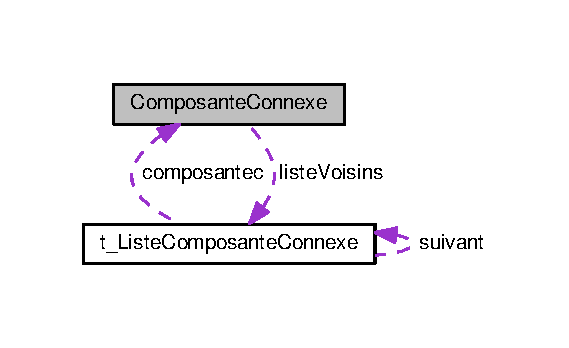
\includegraphics[width=273pt]{struct_composante_connexe__coll__graph}
\end{center}
\end{figure}
\subsection*{Data Fields}
\begin{DoxyCompactItemize}
\item 
\hyperlink{_grille_8c_aa304d0ca681f782b1d7735da33037dd7}{Couleur} \hyperlink{struct_composante_connexe_af0e152d09c13944935e00bef7a3c5111}{couleur}
\item 
\hyperlink{_liste_composante_connexe_8h_a8002dafd0bddf66157ac8cf6e811e4e7}{Liste\+Composante\+Connexe} \hyperlink{struct_composante_connexe_a7c2f71b57647800daa49d283625d1a03}{liste\+Voisins}
\item 
Liste\+Case \hyperlink{struct_composante_connexe_a80edb9cf5135b7f7d3f059d71af4f6cd}{cases}
\end{DoxyCompactItemize}


\subsection{Field Documentation}
\index{Composante\+Connexe@{Composante\+Connexe}!cases@{cases}}
\index{cases@{cases}!Composante\+Connexe@{Composante\+Connexe}}
\subsubsection[{\texorpdfstring{cases}{cases}}]{\setlength{\rightskip}{0pt plus 5cm}Liste\+Case cases}\hypertarget{struct_composante_connexe_a80edb9cf5135b7f7d3f059d71af4f6cd}{}\label{struct_composante_connexe_a80edb9cf5135b7f7d3f059d71af4f6cd}
\index{Composante\+Connexe@{Composante\+Connexe}!couleur@{couleur}}
\index{couleur@{couleur}!Composante\+Connexe@{Composante\+Connexe}}
\subsubsection[{\texorpdfstring{couleur}{couleur}}]{\setlength{\rightskip}{0pt plus 5cm}{\bf Couleur} couleur}\hypertarget{struct_composante_connexe_af0e152d09c13944935e00bef7a3c5111}{}\label{struct_composante_connexe_af0e152d09c13944935e00bef7a3c5111}
\index{Composante\+Connexe@{Composante\+Connexe}!liste\+Voisins@{liste\+Voisins}}
\index{liste\+Voisins@{liste\+Voisins}!Composante\+Connexe@{Composante\+Connexe}}
\subsubsection[{\texorpdfstring{liste\+Voisins}{listeVoisins}}]{\setlength{\rightskip}{0pt plus 5cm}{\bf Liste\+Composante\+Connexe} liste\+Voisins}\hypertarget{struct_composante_connexe_a7c2f71b57647800daa49d283625d1a03}{}\label{struct_composante_connexe_a7c2f71b57647800daa49d283625d1a03}


The documentation for this struct was generated from the following file\+:\begin{DoxyCompactItemize}
\item 
\hyperlink{_composante_connexe_8c}{Composante\+Connexe.\+c}\end{DoxyCompactItemize}

\hypertarget{structt__case}{}\section{t\+\_\+case Struct Reference}
\label{structt__case}\index{t\+\_\+case@{t\+\_\+case}}
\subsection*{Data Fields}
\begin{DoxyCompactItemize}
\item 
int \hyperlink{structt__case_a6150e0515f7202e2fb518f7206ed97dc}{x}
\item 
int \hyperlink{structt__case_a0a2f84ed7838f07779ae24c5a9086d33}{y}
\item 
\hyperlink{_grille_8c_aa304d0ca681f782b1d7735da33037dd7}{Couleur} \hyperlink{structt__case_af0e152d09c13944935e00bef7a3c5111}{couleur}
\end{DoxyCompactItemize}


\subsection{Field Documentation}
\index{t\+\_\+case@{t\+\_\+case}!couleur@{couleur}}
\index{couleur@{couleur}!t\+\_\+case@{t\+\_\+case}}
\subsubsection[{\texorpdfstring{couleur}{couleur}}]{\setlength{\rightskip}{0pt plus 5cm}{\bf Couleur} couleur}\hypertarget{structt__case_af0e152d09c13944935e00bef7a3c5111}{}\label{structt__case_af0e152d09c13944935e00bef7a3c5111}
\index{t\+\_\+case@{t\+\_\+case}!x@{x}}
\index{x@{x}!t\+\_\+case@{t\+\_\+case}}
\subsubsection[{\texorpdfstring{x}{x}}]{\setlength{\rightskip}{0pt plus 5cm}int x}\hypertarget{structt__case_a6150e0515f7202e2fb518f7206ed97dc}{}\label{structt__case_a6150e0515f7202e2fb518f7206ed97dc}
\index{t\+\_\+case@{t\+\_\+case}!y@{y}}
\index{y@{y}!t\+\_\+case@{t\+\_\+case}}
\subsubsection[{\texorpdfstring{y}{y}}]{\setlength{\rightskip}{0pt plus 5cm}int y}\hypertarget{structt__case_a0a2f84ed7838f07779ae24c5a9086d33}{}\label{structt__case_a0a2f84ed7838f07779ae24c5a9086d33}


The documentation for this struct was generated from the following file\+:\begin{DoxyCompactItemize}
\item 
\hyperlink{_grille_8c}{Grille.\+c}\end{DoxyCompactItemize}

\hypertarget{structt___liste_composante_connexe}{}\section{t\+\_\+\+Liste\+Composante\+Connexe Struct Reference}
\label{structt___liste_composante_connexe}\index{t\+\_\+\+Liste\+Composante\+Connexe@{t\+\_\+\+Liste\+Composante\+Connexe}}


Collaboration diagram for t\+\_\+\+Liste\+Composante\+Connexe\+:\nopagebreak
\begin{figure}[H]
\begin{center}
\leavevmode
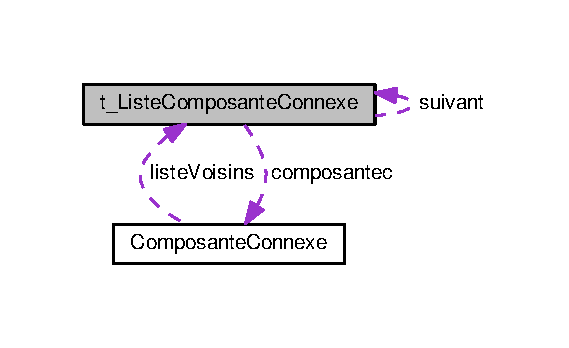
\includegraphics[width=273pt]{structt___liste_composante_connexe__coll__graph}
\end{center}
\end{figure}
\subsection*{Data Fields}
\begin{DoxyCompactItemize}
\item 
\hyperlink{struct_composante_connexe}{Composante\+Connexe} \hyperlink{structt___liste_composante_connexe_a014090efb1c03d5f1036780b1390bc68}{composantec}
\item 
struct \hyperlink{_liste_composante_connexe_8h_a8002dafd0bddf66157ac8cf6e811e4e7}{Liste\+Composante\+Connexe} $\ast$ \hyperlink{structt___liste_composante_connexe_a1de430f247ea74c5770d3fdfcc58d98a}{suivant}
\end{DoxyCompactItemize}


\subsection{Field Documentation}
\index{t\+\_\+\+Liste\+Composante\+Connexe@{t\+\_\+\+Liste\+Composante\+Connexe}!composantec@{composantec}}
\index{composantec@{composantec}!t\+\_\+\+Liste\+Composante\+Connexe@{t\+\_\+\+Liste\+Composante\+Connexe}}
\subsubsection[{\texorpdfstring{composantec}{composantec}}]{\setlength{\rightskip}{0pt plus 5cm}{\bf Composante\+Connexe} composantec}\hypertarget{structt___liste_composante_connexe_a014090efb1c03d5f1036780b1390bc68}{}\label{structt___liste_composante_connexe_a014090efb1c03d5f1036780b1390bc68}
\index{t\+\_\+\+Liste\+Composante\+Connexe@{t\+\_\+\+Liste\+Composante\+Connexe}!suivant@{suivant}}
\index{suivant@{suivant}!t\+\_\+\+Liste\+Composante\+Connexe@{t\+\_\+\+Liste\+Composante\+Connexe}}
\subsubsection[{\texorpdfstring{suivant}{suivant}}]{\setlength{\rightskip}{0pt plus 5cm}struct {\bf Liste\+Composante\+Connexe}$\ast$ suivant}\hypertarget{structt___liste_composante_connexe_a1de430f247ea74c5770d3fdfcc58d98a}{}\label{structt___liste_composante_connexe_a1de430f247ea74c5770d3fdfcc58d98a}


The documentation for this struct was generated from the following file\+:\begin{DoxyCompactItemize}
\item 
\hyperlink{_liste_composante_connexe_8c}{Liste\+Composante\+Connexe.\+c}\end{DoxyCompactItemize}

\chapter{File Documentation}
\hypertarget{_composante_connexe_8c}{}\section{Composante\+Connexe.\+c File Reference}
\label{_composante_connexe_8c}\index{Composante\+Connexe.\+c@{Composante\+Connexe.\+c}}
{\ttfamily \#import \char`\"{}Composante\+Connexe.\+h\char`\"{}}\\*
{\ttfamily \#import \char`\"{}Liste\+Composante\+Connexe.\+h\char`\"{}}\\*
{\ttfamily \#import \char`\"{}Grille.\+h\char`\"{}}\\*
Include dependency graph for Composante\+Connexe.\+c\+:\nopagebreak
\begin{figure}[H]
\begin{center}
\leavevmode
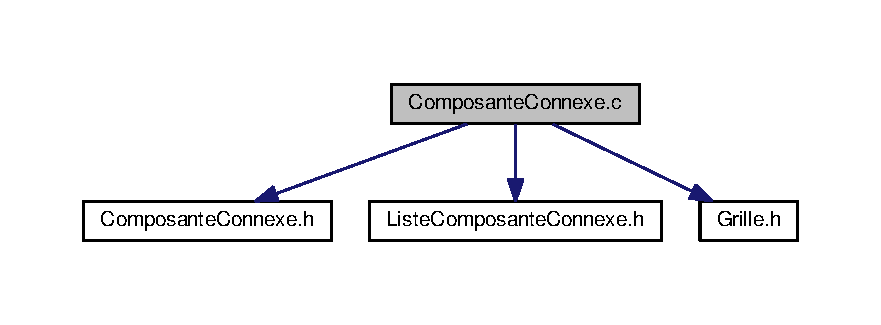
\includegraphics[width=350pt]{_composante_connexe_8c__incl}
\end{center}
\end{figure}
\subsection*{Data Structures}
\begin{DoxyCompactItemize}
\item 
struct \hyperlink{struct_composante_connexe}{Composante\+Connexe}
\end{DoxyCompactItemize}
\subsection*{Functions}
\begin{DoxyCompactItemize}
\item 
struct \hyperlink{struct_composante_connexe}{Composante\+Connexe} \hyperlink{_composante_connexe_8c_a2539fd77b21a1b63ef7934da2f708d93}{init\+Composante\+Connexe} ()
\item 
\hyperlink{struct_composante_connexe}{Composante\+Connexe} \hyperlink{_composante_connexe_8c_a94140137e13e2933373a4c6861e97022}{constructeur\+Composante\+Connexe} (\hyperlink{_grille_8h_adca0b8649254211841dc79ed6c528a86}{Case} emplacement\+Initial, \hyperlink{_grille_8h_adca0b8649254211841dc79ed6c528a86}{Case} $\ast$$\ast$grille)
\item 
void \hyperlink{_composante_connexe_8c_aa5f2aca21f1bf993bf19a6d0dba7cea2}{destructeur\+Composante\+Connexe} (\hyperlink{struct_composante_connexe}{Composante\+Connexe} $\ast$cc)
\item 
Liste\+Case \hyperlink{_composante_connexe_8c_a75fd6ce168c4822da582005a2f1004e5}{get\+Cases\+Composante\+Connexe} (\hyperlink{struct_composante_connexe}{Composante\+Connexe} cc)
\item 
\hyperlink{_liste_composante_connexe_8h_a8002dafd0bddf66157ac8cf6e811e4e7}{Liste\+Composante\+Connexe} \hyperlink{_composante_connexe_8c_a66662d59da551f37d2742dadf1f3dac6}{get\+Composantes\+Voisines\+Composante\+Connexe} (\hyperlink{struct_composante_connexe}{Composante\+Connexe} cc)
\item 
\hyperlink{_grille_8c_aa304d0ca681f782b1d7735da33037dd7}{Couleur} \hyperlink{_composante_connexe_8c_a4eaaa84e02f6185a73a4995e407ef285}{get\+Couleur\+Composante\+Connexe} (\hyperlink{struct_composante_connexe}{Composante\+Connexe} cc)
\item 
Liste\+Case \hyperlink{_composante_connexe_8c_af9cbe5814d9e01c986cc0e7f0610f9e7}{voisins\+Connexes} (\hyperlink{_grille_8h_adca0b8649254211841dc79ed6c528a86}{Case} depart, \hyperlink{_grille_8h_adca0b8649254211841dc79ed6c528a86}{Case} $\ast$$\ast$grille)
\item 
\hyperlink{_liste_composante_connexe_8h_a8002dafd0bddf66157ac8cf6e811e4e7}{Liste\+Composante\+Connexe} \hyperlink{_composante_connexe_8c_afd9654a7f219e2e64937933becbfb340}{liste\+Composante\+Connexe\+Grille} (\hyperlink{_grille_8h_adca0b8649254211841dc79ed6c528a86}{Case} $\ast$$\ast$grille, int taille\+Grille)
\item 
int \hyperlink{_composante_connexe_8c_abaf486ea79c80a4c3514f7a726397eaf}{est\+Indentique} (\hyperlink{struct_composante_connexe}{Composante\+Connexe} cc1, \hyperlink{struct_composante_connexe}{Composante\+Connexe} cc2)
\item 
\hyperlink{_liste_composante_connexe_8h_a8002dafd0bddf66157ac8cf6e811e4e7}{Liste\+Composante\+Connexe} \hyperlink{_composante_connexe_8c_a5d591f19c0cf559dd68e615c19868c44}{definie\+Composantes\+Connexes\+Voisines} (Liste\+Case cases\+Composante\+Connexe, \hyperlink{_grille_8h_adca0b8649254211841dc79ed6c528a86}{Case} $\ast$$\ast$grille)
\item 
\hyperlink{struct_composante_connexe}{Composante\+Connexe} \hyperlink{_composante_connexe_8c_abf849bc5c55c165b6d2497cad6a12137}{changement\+Couleur} (\hyperlink{struct_composante_connexe}{Composante\+Connexe} cc\+Initiale, \hyperlink{_liste_composante_connexe_8h_a8002dafd0bddf66157ac8cf6e811e4e7}{Liste\+Composante\+Connexe} $\ast$toutes\+Composantes\+Connexes, \hyperlink{_grille_8c_aa304d0ca681f782b1d7735da33037dd7}{Couleur} nouvelle\+Couleur)
\end{DoxyCompactItemize}
\subsection*{Variables}
\begin{DoxyCompactItemize}
\item 
\hyperlink{_grille_8c_aa304d0ca681f782b1d7735da33037dd7}{Couleur} \hyperlink{_composante_connexe_8c_af0e152d09c13944935e00bef7a3c5111}{couleur}
\item 
\hyperlink{_liste_composante_connexe_8h_a8002dafd0bddf66157ac8cf6e811e4e7}{Liste\+Composante\+Connexe} \hyperlink{_composante_connexe_8c_a7c2f71b57647800daa49d283625d1a03}{liste\+Voisins}
\item 
Liste\+Case \hyperlink{_composante_connexe_8c_a80edb9cf5135b7f7d3f059d71af4f6cd}{cases}
\end{DoxyCompactItemize}


\subsection{Function Documentation}
\index{Composante\+Connexe.\+c@{Composante\+Connexe.\+c}!changement\+Couleur@{changement\+Couleur}}
\index{changement\+Couleur@{changement\+Couleur}!Composante\+Connexe.\+c@{Composante\+Connexe.\+c}}
\subsubsection[{\texorpdfstring{changement\+Couleur(\+Composante\+Connexe cc\+Initiale, Liste\+Composante\+Connexe $\ast$toutes\+Composantes\+Connexes, Couleur nouvelle\+Couleur)}{changementCouleur(ComposanteConnexe ccInitiale, ListeComposanteConnexe *toutesComposantesConnexes, Couleur nouvelleCouleur)}}]{\setlength{\rightskip}{0pt plus 5cm}{\bf Composante\+Connexe} changement\+Couleur (
\begin{DoxyParamCaption}
\item[{{\bf Composante\+Connexe}}]{cc\+Initiale, }
\item[{{\bf Liste\+Composante\+Connexe} $\ast$}]{toutes\+Composantes\+Connexes, }
\item[{{\bf Couleur}}]{nouvelle\+Couleur}
\end{DoxyParamCaption}
)}\hypertarget{_composante_connexe_8c_abf849bc5c55c165b6d2497cad6a12137}{}\label{_composante_connexe_8c_abf849bc5c55c165b6d2497cad6a12137}
\index{Composante\+Connexe.\+c@{Composante\+Connexe.\+c}!constructeur\+Composante\+Connexe@{constructeur\+Composante\+Connexe}}
\index{constructeur\+Composante\+Connexe@{constructeur\+Composante\+Connexe}!Composante\+Connexe.\+c@{Composante\+Connexe.\+c}}
\subsubsection[{\texorpdfstring{constructeur\+Composante\+Connexe(\+Case emplacement\+Initial, Case $\ast$$\ast$grille)}{constructeurComposanteConnexe(Case emplacementInitial, Case **grille)}}]{\setlength{\rightskip}{0pt plus 5cm}{\bf Composante\+Connexe} constructeur\+Composante\+Connexe (
\begin{DoxyParamCaption}
\item[{{\bf Case}}]{emplacement\+Initial, }
\item[{{\bf Case} $\ast$$\ast$}]{grille}
\end{DoxyParamCaption}
)}\hypertarget{_composante_connexe_8c_a94140137e13e2933373a4c6861e97022}{}\label{_composante_connexe_8c_a94140137e13e2933373a4c6861e97022}
\index{Composante\+Connexe.\+c@{Composante\+Connexe.\+c}!definie\+Composantes\+Connexes\+Voisines@{definie\+Composantes\+Connexes\+Voisines}}
\index{definie\+Composantes\+Connexes\+Voisines@{definie\+Composantes\+Connexes\+Voisines}!Composante\+Connexe.\+c@{Composante\+Connexe.\+c}}
\subsubsection[{\texorpdfstring{definie\+Composantes\+Connexes\+Voisines(\+Liste\+Case cases\+Composante\+Connexe, Case $\ast$$\ast$grille)}{definieComposantesConnexesVoisines(ListeCase casesComposanteConnexe, Case **grille)}}]{\setlength{\rightskip}{0pt plus 5cm}{\bf Liste\+Composante\+Connexe} definie\+Composantes\+Connexes\+Voisines (
\begin{DoxyParamCaption}
\item[{Liste\+Case}]{cases\+Composante\+Connexe, }
\item[{{\bf Case} $\ast$$\ast$}]{grille}
\end{DoxyParamCaption}
)}\hypertarget{_composante_connexe_8c_a5d591f19c0cf559dd68e615c19868c44}{}\label{_composante_connexe_8c_a5d591f19c0cf559dd68e615c19868c44}
\index{Composante\+Connexe.\+c@{Composante\+Connexe.\+c}!destructeur\+Composante\+Connexe@{destructeur\+Composante\+Connexe}}
\index{destructeur\+Composante\+Connexe@{destructeur\+Composante\+Connexe}!Composante\+Connexe.\+c@{Composante\+Connexe.\+c}}
\subsubsection[{\texorpdfstring{destructeur\+Composante\+Connexe(\+Composante\+Connexe $\ast$cc)}{destructeurComposanteConnexe(ComposanteConnexe *cc)}}]{\setlength{\rightskip}{0pt plus 5cm}void destructeur\+Composante\+Connexe (
\begin{DoxyParamCaption}
\item[{{\bf Composante\+Connexe} $\ast$}]{cc}
\end{DoxyParamCaption}
)}\hypertarget{_composante_connexe_8c_aa5f2aca21f1bf993bf19a6d0dba7cea2}{}\label{_composante_connexe_8c_aa5f2aca21f1bf993bf19a6d0dba7cea2}
\index{Composante\+Connexe.\+c@{Composante\+Connexe.\+c}!est\+Indentique@{est\+Indentique}}
\index{est\+Indentique@{est\+Indentique}!Composante\+Connexe.\+c@{Composante\+Connexe.\+c}}
\subsubsection[{\texorpdfstring{est\+Indentique(\+Composante\+Connexe cc1, Composante\+Connexe cc2)}{estIndentique(ComposanteConnexe cc1, ComposanteConnexe cc2)}}]{\setlength{\rightskip}{0pt plus 5cm}int est\+Indentique (
\begin{DoxyParamCaption}
\item[{{\bf Composante\+Connexe}}]{cc1, }
\item[{{\bf Composante\+Connexe}}]{cc2}
\end{DoxyParamCaption}
)}\hypertarget{_composante_connexe_8c_abaf486ea79c80a4c3514f7a726397eaf}{}\label{_composante_connexe_8c_abaf486ea79c80a4c3514f7a726397eaf}
\index{Composante\+Connexe.\+c@{Composante\+Connexe.\+c}!get\+Cases\+Composante\+Connexe@{get\+Cases\+Composante\+Connexe}}
\index{get\+Cases\+Composante\+Connexe@{get\+Cases\+Composante\+Connexe}!Composante\+Connexe.\+c@{Composante\+Connexe.\+c}}
\subsubsection[{\texorpdfstring{get\+Cases\+Composante\+Connexe(\+Composante\+Connexe cc)}{getCasesComposanteConnexe(ComposanteConnexe cc)}}]{\setlength{\rightskip}{0pt plus 5cm}Liste\+Case get\+Cases\+Composante\+Connexe (
\begin{DoxyParamCaption}
\item[{{\bf Composante\+Connexe}}]{cc}
\end{DoxyParamCaption}
)}\hypertarget{_composante_connexe_8c_a75fd6ce168c4822da582005a2f1004e5}{}\label{_composante_connexe_8c_a75fd6ce168c4822da582005a2f1004e5}
\index{Composante\+Connexe.\+c@{Composante\+Connexe.\+c}!get\+Composantes\+Voisines\+Composante\+Connexe@{get\+Composantes\+Voisines\+Composante\+Connexe}}
\index{get\+Composantes\+Voisines\+Composante\+Connexe@{get\+Composantes\+Voisines\+Composante\+Connexe}!Composante\+Connexe.\+c@{Composante\+Connexe.\+c}}
\subsubsection[{\texorpdfstring{get\+Composantes\+Voisines\+Composante\+Connexe(\+Composante\+Connexe cc)}{getComposantesVoisinesComposanteConnexe(ComposanteConnexe cc)}}]{\setlength{\rightskip}{0pt plus 5cm}{\bf Liste\+Composante\+Connexe} get\+Composantes\+Voisines\+Composante\+Connexe (
\begin{DoxyParamCaption}
\item[{{\bf Composante\+Connexe}}]{cc}
\end{DoxyParamCaption}
)}\hypertarget{_composante_connexe_8c_a66662d59da551f37d2742dadf1f3dac6}{}\label{_composante_connexe_8c_a66662d59da551f37d2742dadf1f3dac6}
\index{Composante\+Connexe.\+c@{Composante\+Connexe.\+c}!get\+Couleur\+Composante\+Connexe@{get\+Couleur\+Composante\+Connexe}}
\index{get\+Couleur\+Composante\+Connexe@{get\+Couleur\+Composante\+Connexe}!Composante\+Connexe.\+c@{Composante\+Connexe.\+c}}
\subsubsection[{\texorpdfstring{get\+Couleur\+Composante\+Connexe(\+Composante\+Connexe cc)}{getCouleurComposanteConnexe(ComposanteConnexe cc)}}]{\setlength{\rightskip}{0pt plus 5cm}{\bf Couleur} get\+Couleur\+Composante\+Connexe (
\begin{DoxyParamCaption}
\item[{{\bf Composante\+Connexe}}]{cc}
\end{DoxyParamCaption}
)}\hypertarget{_composante_connexe_8c_a4eaaa84e02f6185a73a4995e407ef285}{}\label{_composante_connexe_8c_a4eaaa84e02f6185a73a4995e407ef285}
\index{Composante\+Connexe.\+c@{Composante\+Connexe.\+c}!init\+Composante\+Connexe@{init\+Composante\+Connexe}}
\index{init\+Composante\+Connexe@{init\+Composante\+Connexe}!Composante\+Connexe.\+c@{Composante\+Connexe.\+c}}
\subsubsection[{\texorpdfstring{init\+Composante\+Connexe()}{initComposanteConnexe()}}]{\setlength{\rightskip}{0pt plus 5cm}struct {\bf Composante\+Connexe} init\+Composante\+Connexe (
\begin{DoxyParamCaption}
{}
\end{DoxyParamCaption}
)}\hypertarget{_composante_connexe_8c_a2539fd77b21a1b63ef7934da2f708d93}{}\label{_composante_connexe_8c_a2539fd77b21a1b63ef7934da2f708d93}
\index{Composante\+Connexe.\+c@{Composante\+Connexe.\+c}!liste\+Composante\+Connexe\+Grille@{liste\+Composante\+Connexe\+Grille}}
\index{liste\+Composante\+Connexe\+Grille@{liste\+Composante\+Connexe\+Grille}!Composante\+Connexe.\+c@{Composante\+Connexe.\+c}}
\subsubsection[{\texorpdfstring{liste\+Composante\+Connexe\+Grille(\+Case $\ast$$\ast$grille, int taille\+Grille)}{listeComposanteConnexeGrille(Case **grille, int tailleGrille)}}]{\setlength{\rightskip}{0pt plus 5cm}{\bf Liste\+Composante\+Connexe} liste\+Composante\+Connexe\+Grille (
\begin{DoxyParamCaption}
\item[{{\bf Case} $\ast$$\ast$}]{grille, }
\item[{int}]{taille\+Grille}
\end{DoxyParamCaption}
)}\hypertarget{_composante_connexe_8c_afd9654a7f219e2e64937933becbfb340}{}\label{_composante_connexe_8c_afd9654a7f219e2e64937933becbfb340}
\index{Composante\+Connexe.\+c@{Composante\+Connexe.\+c}!voisins\+Connexes@{voisins\+Connexes}}
\index{voisins\+Connexes@{voisins\+Connexes}!Composante\+Connexe.\+c@{Composante\+Connexe.\+c}}
\subsubsection[{\texorpdfstring{voisins\+Connexes(\+Case depart, Case $\ast$$\ast$grille)}{voisinsConnexes(Case depart, Case **grille)}}]{\setlength{\rightskip}{0pt plus 5cm}Liste\+Case voisins\+Connexes (
\begin{DoxyParamCaption}
\item[{{\bf Case}}]{depart, }
\item[{{\bf Case} $\ast$$\ast$}]{grille}
\end{DoxyParamCaption}
)}\hypertarget{_composante_connexe_8c_af9cbe5814d9e01c986cc0e7f0610f9e7}{}\label{_composante_connexe_8c_af9cbe5814d9e01c986cc0e7f0610f9e7}


\subsection{Variable Documentation}
\index{Composante\+Connexe.\+c@{Composante\+Connexe.\+c}!cases@{cases}}
\index{cases@{cases}!Composante\+Connexe.\+c@{Composante\+Connexe.\+c}}
\subsubsection[{\texorpdfstring{cases}{cases}}]{\setlength{\rightskip}{0pt plus 5cm}Liste\+Case cases}\hypertarget{_composante_connexe_8c_a80edb9cf5135b7f7d3f059d71af4f6cd}{}\label{_composante_connexe_8c_a80edb9cf5135b7f7d3f059d71af4f6cd}
\index{Composante\+Connexe.\+c@{Composante\+Connexe.\+c}!couleur@{couleur}}
\index{couleur@{couleur}!Composante\+Connexe.\+c@{Composante\+Connexe.\+c}}
\subsubsection[{\texorpdfstring{couleur}{couleur}}]{\setlength{\rightskip}{0pt plus 5cm}{\bf Couleur} couleur}\hypertarget{_composante_connexe_8c_af0e152d09c13944935e00bef7a3c5111}{}\label{_composante_connexe_8c_af0e152d09c13944935e00bef7a3c5111}
\index{Composante\+Connexe.\+c@{Composante\+Connexe.\+c}!liste\+Voisins@{liste\+Voisins}}
\index{liste\+Voisins@{liste\+Voisins}!Composante\+Connexe.\+c@{Composante\+Connexe.\+c}}
\subsubsection[{\texorpdfstring{liste\+Voisins}{listeVoisins}}]{\setlength{\rightskip}{0pt plus 5cm}{\bf Liste\+Composante\+Connexe} liste\+Voisins}\hypertarget{_composante_connexe_8c_a7c2f71b57647800daa49d283625d1a03}{}\label{_composante_connexe_8c_a7c2f71b57647800daa49d283625d1a03}

\hypertarget{_composante_connexe_8h}{}\section{Composante\+Connexe.\+h File Reference}
\label{_composante_connexe_8h}\index{Composante\+Connexe.\+h@{Composante\+Connexe.\+h}}
This graph shows which files directly or indirectly include this file\+:\nopagebreak
\begin{figure}[H]
\begin{center}
\leavevmode
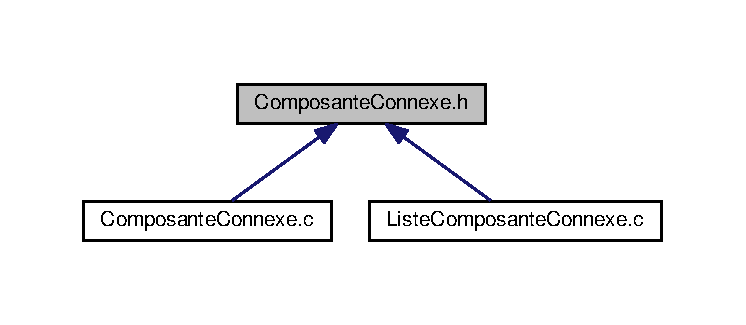
\includegraphics[width=350pt]{_composante_connexe_8h__dep__incl}
\end{center}
\end{figure}
\subsection*{Typedefs}
\begin{DoxyCompactItemize}
\item 
typedef struct \hyperlink{struct_composante_connexe}{Composante\+Connexe} \hyperlink{_composante_connexe_8h_a5fb75d45d33d42158de143d5bc978851}{Composante\+Connexe}
\end{DoxyCompactItemize}
\subsection*{Functions}
\begin{DoxyCompactItemize}
\item 
\hyperlink{struct_composante_connexe}{Composante\+Connexe} \hyperlink{_composante_connexe_8h_aa3731bdba830e80c38f5360e96d77571}{init\+Composante\+Connexe} ()
\item 
\hyperlink{struct_composante_connexe}{Composante\+Connexe} \hyperlink{_composante_connexe_8h_a94140137e13e2933373a4c6861e97022}{constructeur\+Composante\+Connexe} (\hyperlink{_grille_8h_adca0b8649254211841dc79ed6c528a86}{Case} emplacement\+Initial, \hyperlink{_grille_8h_adca0b8649254211841dc79ed6c528a86}{Case} $\ast$$\ast$grille)
\item 
void \hyperlink{_composante_connexe_8h_aa5f2aca21f1bf993bf19a6d0dba7cea2}{destructeur\+Composante\+Connexe} (\hyperlink{struct_composante_connexe}{Composante\+Connexe} $\ast$cc)
\item 
Liste\+Case \hyperlink{_composante_connexe_8h_a75fd6ce168c4822da582005a2f1004e5}{get\+Cases\+Composante\+Connexe} (\hyperlink{struct_composante_connexe}{Composante\+Connexe} cc)
\item 
\hyperlink{_liste_composante_connexe_8h_a8002dafd0bddf66157ac8cf6e811e4e7}{Liste\+Composante\+Connexe} \hyperlink{_composante_connexe_8h_a66662d59da551f37d2742dadf1f3dac6}{get\+Composantes\+Voisines\+Composante\+Connexe} (\hyperlink{struct_composante_connexe}{Composante\+Connexe} cc)
\item 
\hyperlink{_grille_8c_aa304d0ca681f782b1d7735da33037dd7}{Couleur} \hyperlink{_composante_connexe_8h_a4eaaa84e02f6185a73a4995e407ef285}{get\+Couleur\+Composante\+Connexe} (\hyperlink{struct_composante_connexe}{Composante\+Connexe} cc)
\item 
Liste\+Case \hyperlink{_composante_connexe_8h_ab3aa262f92e89899e25cf8a03eba89ec}{voisins\+Connexes} (\hyperlink{_grille_8h_adca0b8649254211841dc79ed6c528a86}{Case} emplacement\+Initial)
\item 
\hyperlink{_liste_composante_connexe_8h_a8002dafd0bddf66157ac8cf6e811e4e7}{Liste\+Composante\+Connexe} \hyperlink{_composante_connexe_8h_afd9654a7f219e2e64937933becbfb340}{liste\+Composante\+Connexe\+Grille} (\hyperlink{_grille_8h_adca0b8649254211841dc79ed6c528a86}{Case} $\ast$$\ast$grille, int taille\+Grille)
\item 
int \hyperlink{_composante_connexe_8h_abaf486ea79c80a4c3514f7a726397eaf}{est\+Indentique} (\hyperlink{struct_composante_connexe}{Composante\+Connexe} cc1, \hyperlink{struct_composante_connexe}{Composante\+Connexe} cc2)
\item 
\hyperlink{_liste_composante_connexe_8h_a8002dafd0bddf66157ac8cf6e811e4e7}{Liste\+Composante\+Connexe} \hyperlink{_composante_connexe_8h_ac782a101a4695c5ee3af7e7b07c137dc}{definie\+Composantes\+Connexes\+Voisines} (Liste\+Case cases\+Composante\+Connexe, \hyperlink{_liste_composante_connexe_8h_a8002dafd0bddf66157ac8cf6e811e4e7}{Liste\+Composante\+Connexe} liste\+CC, \hyperlink{_grille_8h_adca0b8649254211841dc79ed6c528a86}{Case} $\ast$$\ast$grille)
\item 
\hyperlink{struct_composante_connexe}{Composante\+Connexe} \hyperlink{_composante_connexe_8h_abf849bc5c55c165b6d2497cad6a12137}{changement\+Couleur} (\hyperlink{struct_composante_connexe}{Composante\+Connexe} cc\+Initiale, \hyperlink{_liste_composante_connexe_8h_a8002dafd0bddf66157ac8cf6e811e4e7}{Liste\+Composante\+Connexe} $\ast$toutes\+Composantes\+Connexes, \hyperlink{_grille_8c_aa304d0ca681f782b1d7735da33037dd7}{Couleur} nouvelle\+Couleur)
\end{DoxyCompactItemize}


\subsection{Typedef Documentation}
\index{Composante\+Connexe.\+h@{Composante\+Connexe.\+h}!Composante\+Connexe@{Composante\+Connexe}}
\index{Composante\+Connexe@{Composante\+Connexe}!Composante\+Connexe.\+h@{Composante\+Connexe.\+h}}
\subsubsection[{\texorpdfstring{Composante\+Connexe}{ComposanteConnexe}}]{\setlength{\rightskip}{0pt plus 5cm}typedef struct {\bf Composante\+Connexe} {\bf Composante\+Connexe}}\hypertarget{_composante_connexe_8h_a5fb75d45d33d42158de143d5bc978851}{}\label{_composante_connexe_8h_a5fb75d45d33d42158de143d5bc978851}


\subsection{Function Documentation}
\index{Composante\+Connexe.\+h@{Composante\+Connexe.\+h}!changement\+Couleur@{changement\+Couleur}}
\index{changement\+Couleur@{changement\+Couleur}!Composante\+Connexe.\+h@{Composante\+Connexe.\+h}}
\subsubsection[{\texorpdfstring{changement\+Couleur(\+Composante\+Connexe cc\+Initiale, Liste\+Composante\+Connexe $\ast$toutes\+Composantes\+Connexes, Couleur nouvelle\+Couleur)}{changementCouleur(ComposanteConnexe ccInitiale, ListeComposanteConnexe *toutesComposantesConnexes, Couleur nouvelleCouleur)}}]{\setlength{\rightskip}{0pt plus 5cm}{\bf Composante\+Connexe} changement\+Couleur (
\begin{DoxyParamCaption}
\item[{{\bf Composante\+Connexe}}]{cc\+Initiale, }
\item[{{\bf Liste\+Composante\+Connexe} $\ast$}]{toutes\+Composantes\+Connexes, }
\item[{{\bf Couleur}}]{nouvelle\+Couleur}
\end{DoxyParamCaption}
)}\hypertarget{_composante_connexe_8h_abf849bc5c55c165b6d2497cad6a12137}{}\label{_composante_connexe_8h_abf849bc5c55c165b6d2497cad6a12137}
\index{Composante\+Connexe.\+h@{Composante\+Connexe.\+h}!constructeur\+Composante\+Connexe@{constructeur\+Composante\+Connexe}}
\index{constructeur\+Composante\+Connexe@{constructeur\+Composante\+Connexe}!Composante\+Connexe.\+h@{Composante\+Connexe.\+h}}
\subsubsection[{\texorpdfstring{constructeur\+Composante\+Connexe(\+Case emplacement\+Initial, Case $\ast$$\ast$grille)}{constructeurComposanteConnexe(Case emplacementInitial, Case **grille)}}]{\setlength{\rightskip}{0pt plus 5cm}{\bf Composante\+Connexe} constructeur\+Composante\+Connexe (
\begin{DoxyParamCaption}
\item[{{\bf Case}}]{emplacement\+Initial, }
\item[{{\bf Case} $\ast$$\ast$}]{grille}
\end{DoxyParamCaption}
)}\hypertarget{_composante_connexe_8h_a94140137e13e2933373a4c6861e97022}{}\label{_composante_connexe_8h_a94140137e13e2933373a4c6861e97022}
\index{Composante\+Connexe.\+h@{Composante\+Connexe.\+h}!definie\+Composantes\+Connexes\+Voisines@{definie\+Composantes\+Connexes\+Voisines}}
\index{definie\+Composantes\+Connexes\+Voisines@{definie\+Composantes\+Connexes\+Voisines}!Composante\+Connexe.\+h@{Composante\+Connexe.\+h}}
\subsubsection[{\texorpdfstring{definie\+Composantes\+Connexes\+Voisines(\+Liste\+Case cases\+Composante\+Connexe, Liste\+Composante\+Connexe liste\+C\+C, Case $\ast$$\ast$grille)}{definieComposantesConnexesVoisines(ListeCase casesComposanteConnexe, ListeComposanteConnexe listeCC, Case **grille)}}]{\setlength{\rightskip}{0pt plus 5cm}{\bf Liste\+Composante\+Connexe} definie\+Composantes\+Connexes\+Voisines (
\begin{DoxyParamCaption}
\item[{Liste\+Case}]{cases\+Composante\+Connexe, }
\item[{{\bf Liste\+Composante\+Connexe}}]{liste\+CC, }
\item[{{\bf Case} $\ast$$\ast$}]{grille}
\end{DoxyParamCaption}
)}\hypertarget{_composante_connexe_8h_ac782a101a4695c5ee3af7e7b07c137dc}{}\label{_composante_connexe_8h_ac782a101a4695c5ee3af7e7b07c137dc}
\index{Composante\+Connexe.\+h@{Composante\+Connexe.\+h}!destructeur\+Composante\+Connexe@{destructeur\+Composante\+Connexe}}
\index{destructeur\+Composante\+Connexe@{destructeur\+Composante\+Connexe}!Composante\+Connexe.\+h@{Composante\+Connexe.\+h}}
\subsubsection[{\texorpdfstring{destructeur\+Composante\+Connexe(\+Composante\+Connexe $\ast$cc)}{destructeurComposanteConnexe(ComposanteConnexe *cc)}}]{\setlength{\rightskip}{0pt plus 5cm}void destructeur\+Composante\+Connexe (
\begin{DoxyParamCaption}
\item[{{\bf Composante\+Connexe} $\ast$}]{cc}
\end{DoxyParamCaption}
)}\hypertarget{_composante_connexe_8h_aa5f2aca21f1bf993bf19a6d0dba7cea2}{}\label{_composante_connexe_8h_aa5f2aca21f1bf993bf19a6d0dba7cea2}
\index{Composante\+Connexe.\+h@{Composante\+Connexe.\+h}!est\+Indentique@{est\+Indentique}}
\index{est\+Indentique@{est\+Indentique}!Composante\+Connexe.\+h@{Composante\+Connexe.\+h}}
\subsubsection[{\texorpdfstring{est\+Indentique(\+Composante\+Connexe cc1, Composante\+Connexe cc2)}{estIndentique(ComposanteConnexe cc1, ComposanteConnexe cc2)}}]{\setlength{\rightskip}{0pt plus 5cm}int est\+Indentique (
\begin{DoxyParamCaption}
\item[{{\bf Composante\+Connexe}}]{cc1, }
\item[{{\bf Composante\+Connexe}}]{cc2}
\end{DoxyParamCaption}
)}\hypertarget{_composante_connexe_8h_abaf486ea79c80a4c3514f7a726397eaf}{}\label{_composante_connexe_8h_abaf486ea79c80a4c3514f7a726397eaf}
\index{Composante\+Connexe.\+h@{Composante\+Connexe.\+h}!get\+Cases\+Composante\+Connexe@{get\+Cases\+Composante\+Connexe}}
\index{get\+Cases\+Composante\+Connexe@{get\+Cases\+Composante\+Connexe}!Composante\+Connexe.\+h@{Composante\+Connexe.\+h}}
\subsubsection[{\texorpdfstring{get\+Cases\+Composante\+Connexe(\+Composante\+Connexe cc)}{getCasesComposanteConnexe(ComposanteConnexe cc)}}]{\setlength{\rightskip}{0pt plus 5cm}Liste\+Case get\+Cases\+Composante\+Connexe (
\begin{DoxyParamCaption}
\item[{{\bf Composante\+Connexe}}]{cc}
\end{DoxyParamCaption}
)}\hypertarget{_composante_connexe_8h_a75fd6ce168c4822da582005a2f1004e5}{}\label{_composante_connexe_8h_a75fd6ce168c4822da582005a2f1004e5}
\index{Composante\+Connexe.\+h@{Composante\+Connexe.\+h}!get\+Composantes\+Voisines\+Composante\+Connexe@{get\+Composantes\+Voisines\+Composante\+Connexe}}
\index{get\+Composantes\+Voisines\+Composante\+Connexe@{get\+Composantes\+Voisines\+Composante\+Connexe}!Composante\+Connexe.\+h@{Composante\+Connexe.\+h}}
\subsubsection[{\texorpdfstring{get\+Composantes\+Voisines\+Composante\+Connexe(\+Composante\+Connexe cc)}{getComposantesVoisinesComposanteConnexe(ComposanteConnexe cc)}}]{\setlength{\rightskip}{0pt plus 5cm}{\bf Liste\+Composante\+Connexe} get\+Composantes\+Voisines\+Composante\+Connexe (
\begin{DoxyParamCaption}
\item[{{\bf Composante\+Connexe}}]{cc}
\end{DoxyParamCaption}
)}\hypertarget{_composante_connexe_8h_a66662d59da551f37d2742dadf1f3dac6}{}\label{_composante_connexe_8h_a66662d59da551f37d2742dadf1f3dac6}
\index{Composante\+Connexe.\+h@{Composante\+Connexe.\+h}!get\+Couleur\+Composante\+Connexe@{get\+Couleur\+Composante\+Connexe}}
\index{get\+Couleur\+Composante\+Connexe@{get\+Couleur\+Composante\+Connexe}!Composante\+Connexe.\+h@{Composante\+Connexe.\+h}}
\subsubsection[{\texorpdfstring{get\+Couleur\+Composante\+Connexe(\+Composante\+Connexe cc)}{getCouleurComposanteConnexe(ComposanteConnexe cc)}}]{\setlength{\rightskip}{0pt plus 5cm}{\bf Couleur} get\+Couleur\+Composante\+Connexe (
\begin{DoxyParamCaption}
\item[{{\bf Composante\+Connexe}}]{cc}
\end{DoxyParamCaption}
)}\hypertarget{_composante_connexe_8h_a4eaaa84e02f6185a73a4995e407ef285}{}\label{_composante_connexe_8h_a4eaaa84e02f6185a73a4995e407ef285}
\index{Composante\+Connexe.\+h@{Composante\+Connexe.\+h}!init\+Composante\+Connexe@{init\+Composante\+Connexe}}
\index{init\+Composante\+Connexe@{init\+Composante\+Connexe}!Composante\+Connexe.\+h@{Composante\+Connexe.\+h}}
\subsubsection[{\texorpdfstring{init\+Composante\+Connexe()}{initComposanteConnexe()}}]{\setlength{\rightskip}{0pt plus 5cm}{\bf Composante\+Connexe} init\+Composante\+Connexe (
\begin{DoxyParamCaption}
{}
\end{DoxyParamCaption}
)}\hypertarget{_composante_connexe_8h_aa3731bdba830e80c38f5360e96d77571}{}\label{_composante_connexe_8h_aa3731bdba830e80c38f5360e96d77571}
\index{Composante\+Connexe.\+h@{Composante\+Connexe.\+h}!liste\+Composante\+Connexe\+Grille@{liste\+Composante\+Connexe\+Grille}}
\index{liste\+Composante\+Connexe\+Grille@{liste\+Composante\+Connexe\+Grille}!Composante\+Connexe.\+h@{Composante\+Connexe.\+h}}
\subsubsection[{\texorpdfstring{liste\+Composante\+Connexe\+Grille(\+Case $\ast$$\ast$grille, int taille\+Grille)}{listeComposanteConnexeGrille(Case **grille, int tailleGrille)}}]{\setlength{\rightskip}{0pt plus 5cm}{\bf Liste\+Composante\+Connexe} liste\+Composante\+Connexe\+Grille (
\begin{DoxyParamCaption}
\item[{{\bf Case} $\ast$$\ast$}]{grille, }
\item[{int}]{taille\+Grille}
\end{DoxyParamCaption}
)}\hypertarget{_composante_connexe_8h_afd9654a7f219e2e64937933becbfb340}{}\label{_composante_connexe_8h_afd9654a7f219e2e64937933becbfb340}
\index{Composante\+Connexe.\+h@{Composante\+Connexe.\+h}!voisins\+Connexes@{voisins\+Connexes}}
\index{voisins\+Connexes@{voisins\+Connexes}!Composante\+Connexe.\+h@{Composante\+Connexe.\+h}}
\subsubsection[{\texorpdfstring{voisins\+Connexes(\+Case emplacement\+Initial)}{voisinsConnexes(Case emplacementInitial)}}]{\setlength{\rightskip}{0pt plus 5cm}Liste\+Case voisins\+Connexes (
\begin{DoxyParamCaption}
\item[{{\bf Case}}]{emplacement\+Initial}
\end{DoxyParamCaption}
)}\hypertarget{_composante_connexe_8h_ab3aa262f92e89899e25cf8a03eba89ec}{}\label{_composante_connexe_8h_ab3aa262f92e89899e25cf8a03eba89ec}

\hypertarget{_grille_8c}{}\section{Grille.\+c File Reference}
\label{_grille_8c}\index{Grille.\+c@{Grille.\+c}}
{\ttfamily \#include $<$stdio.\+h$>$}\\*
{\ttfamily \#include $<$stdlib.\+h$>$}\\*
{\ttfamily \#include $<$math.\+h$>$}\\*
{\ttfamily \#include $<$cunit.\+h$>$}\\*
Include dependency graph for Grille.\+c\+:\nopagebreak
\begin{figure}[H]
\begin{center}
\leavevmode
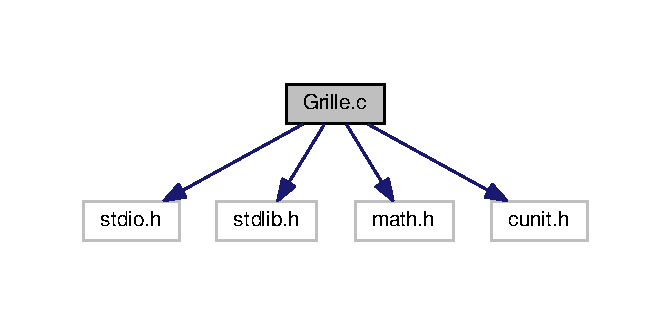
\includegraphics[width=322pt]{_grille_8c__incl}
\end{center}
\end{figure}
\subsection*{Data Structures}
\begin{DoxyCompactItemize}
\item 
struct \hyperlink{structt__case}{t\+\_\+case}
\end{DoxyCompactItemize}
\subsection*{Enumerations}
\begin{DoxyCompactItemize}
\item 
enum \hyperlink{_grille_8c_aa304d0ca681f782b1d7735da33037dd7}{Couleur} \{ \\*
\hyperlink{_grille_8c_aa304d0ca681f782b1d7735da33037dd7a3f2a77ecd272aa6d6b5902faa5e5fc68}{B}, 
\hyperlink{_grille_8c_aa304d0ca681f782b1d7735da33037dd7a28f41f1144eee94834387e9a6a088bc1}{V}, 
\hyperlink{_grille_8c_aa304d0ca681f782b1d7735da33037dd7a1784b1a3d7cbd43c45ff82c72d05e4ae}{R}, 
\hyperlink{_grille_8c_aa304d0ca681f782b1d7735da33037dd7a03605500b0c55f3d95874e8edfcf4e30}{J}, 
\\*
\hyperlink{_grille_8c_aa304d0ca681f782b1d7735da33037dd7a51ca6c63d97347ee58cc7da59ab6994b}{M}, 
\hyperlink{_grille_8c_aa304d0ca681f782b1d7735da33037dd7a2fe993340f6abb2234e543cd427df70b}{G}, 
\hyperlink{_grille_8h_aa304d0ca681f782b1d7735da33037dd7a3f2a77ecd272aa6d6b5902faa5e5fc68}{B}, 
\hyperlink{_grille_8h_aa304d0ca681f782b1d7735da33037dd7a28f41f1144eee94834387e9a6a088bc1}{V}, 
\\*
\hyperlink{_grille_8h_aa304d0ca681f782b1d7735da33037dd7a1784b1a3d7cbd43c45ff82c72d05e4ae}{R}, 
\hyperlink{_grille_8h_aa304d0ca681f782b1d7735da33037dd7a03605500b0c55f3d95874e8edfcf4e30}{J}, 
\hyperlink{_grille_8h_aa304d0ca681f782b1d7735da33037dd7a51ca6c63d97347ee58cc7da59ab6994b}{M}, 
\hyperlink{_grille_8h_aa304d0ca681f782b1d7735da33037dd7a2fe993340f6abb2234e543cd427df70b}{G}
 \}
\end{DoxyCompactItemize}
\subsection*{Functions}
\begin{DoxyCompactItemize}
\item 
int \hyperlink{_grille_8c_a802e561ca78785bfb07308847f57decc}{get\+X\+Case} (\hyperlink{_grille_8h_adca0b8649254211841dc79ed6c528a86}{Case} test)
\begin{DoxyCompactList}\small\item\em Récupère l\textquotesingle{}abscisse de la case considérée. \end{DoxyCompactList}\item 
int \hyperlink{_grille_8c_acfff6837eafd46f5269db9399503ae0c}{get\+Y\+Case} (\hyperlink{_grille_8h_adca0b8649254211841dc79ed6c528a86}{Case} test)
\begin{DoxyCompactList}\small\item\em Récupère l\textquotesingle{}ordonnée de la case considérée. \end{DoxyCompactList}\item 
int \hyperlink{_grille_8c_a1f67bc9aaa3d2b2e18bc56cbd64e9db4}{get\+Couleur\+Case} (\hyperlink{_grille_8h_adca0b8649254211841dc79ed6c528a86}{Case} test)
\begin{DoxyCompactList}\small\item\em Récupère la couleur de la case considérée. \end{DoxyCompactList}\item 
void \hyperlink{_grille_8c_afa2e284e68787b2997383a31eb764b97}{set\+Couleur} (\hyperlink{_grille_8h_adca0b8649254211841dc79ed6c528a86}{Case} $\ast$test, \hyperlink{_grille_8c_aa304d0ca681f782b1d7735da33037dd7}{Couleur} c)
\begin{DoxyCompactList}\small\item\em Change la couleur de la case considérée par la couleur en paramètre. \end{DoxyCompactList}\item 
\hyperlink{_grille_8h_adca0b8649254211841dc79ed6c528a86}{Case} $\ast$$\ast$ \hyperlink{_grille_8c_a1b8be80378b6a5b3fca696f93d67e1a9}{tableau\+Vide} (int n)
\begin{DoxyCompactList}\small\item\em Initialise un tableau vide de taille n. \end{DoxyCompactList}\item 
void \hyperlink{_grille_8c_a63924a00bcf27e9d394076c4659ae55c}{liberation\+Grille} (\hyperlink{_grille_8h_adca0b8649254211841dc79ed6c528a86}{Case} $\ast$$\ast$tab, int taille)
\begin{DoxyCompactList}\small\item\em Libère l\textquotesingle{}espace mémoire occupé par la grille. \end{DoxyCompactList}\item 
\hyperlink{_grille_8c_aa304d0ca681f782b1d7735da33037dd7}{Couleur} $\ast$$\ast$ \hyperlink{_grille_8c_af90a8c5a6dfed19c42a57f0ca19daf81}{remplissage\+Aleatoire} (int n)
\begin{DoxyCompactList}\small\item\em Fonction de remplissage aléatoire du tableau. \end{DoxyCompactList}\item 
\hyperlink{_grille_8c_aa304d0ca681f782b1d7735da33037dd7}{Couleur} $\ast$$\ast$ \hyperlink{_grille_8c_afd85b7e73c3be3858db354ee7f802683}{remplissage\+Fichier} (char $\ast$text)
\begin{DoxyCompactList}\small\item\em Crée un tableau de couleur à partir d\textquotesingle{}un fichier. Le fichier doit contenir des chaines de caractères contenant un retour à la ligne au bout de chaque ligne. \end{DoxyCompactList}\end{DoxyCompactItemize}
\subsection*{Variables}
\begin{DoxyCompactItemize}
\item 
enum \hyperlink{_grille_8c_aa304d0ca681f782b1d7735da33037dd7}{Couleur} \hyperlink{_grille_8c_a834ed0e52397f713642e488e87508c9e}{init\+Composante\+Connexe}
\end{DoxyCompactItemize}


\subsection{Enumeration Type Documentation}
\index{Grille.\+c@{Grille.\+c}!Couleur@{Couleur}}
\index{Couleur@{Couleur}!Grille.\+c@{Grille.\+c}}
\subsubsection[{\texorpdfstring{Couleur}{Couleur}}]{\setlength{\rightskip}{0pt plus 5cm}enum {\bf Couleur}}\hypertarget{_grille_8c_aa304d0ca681f782b1d7735da33037dd7}{}\label{_grille_8c_aa304d0ca681f782b1d7735da33037dd7}
\begin{Desc}
\item[Enumerator]\par
\begin{description}
\index{B@{B}!Grille.\+c@{Grille.\+c}}\index{Grille.\+c@{Grille.\+c}!B@{B}}\item[{\em 
B\hypertarget{_grille_8c_aa304d0ca681f782b1d7735da33037dd7a3f2a77ecd272aa6d6b5902faa5e5fc68}{}\label{_grille_8c_aa304d0ca681f782b1d7735da33037dd7a3f2a77ecd272aa6d6b5902faa5e5fc68}
}]\index{V@{V}!Grille.\+c@{Grille.\+c}}\index{Grille.\+c@{Grille.\+c}!V@{V}}\item[{\em 
V\hypertarget{_grille_8c_aa304d0ca681f782b1d7735da33037dd7a28f41f1144eee94834387e9a6a088bc1}{}\label{_grille_8c_aa304d0ca681f782b1d7735da33037dd7a28f41f1144eee94834387e9a6a088bc1}
}]\index{R@{R}!Grille.\+c@{Grille.\+c}}\index{Grille.\+c@{Grille.\+c}!R@{R}}\item[{\em 
R\hypertarget{_grille_8c_aa304d0ca681f782b1d7735da33037dd7a1784b1a3d7cbd43c45ff82c72d05e4ae}{}\label{_grille_8c_aa304d0ca681f782b1d7735da33037dd7a1784b1a3d7cbd43c45ff82c72d05e4ae}
}]\index{J@{J}!Grille.\+c@{Grille.\+c}}\index{Grille.\+c@{Grille.\+c}!J@{J}}\item[{\em 
J\hypertarget{_grille_8c_aa304d0ca681f782b1d7735da33037dd7a03605500b0c55f3d95874e8edfcf4e30}{}\label{_grille_8c_aa304d0ca681f782b1d7735da33037dd7a03605500b0c55f3d95874e8edfcf4e30}
}]\index{M@{M}!Grille.\+c@{Grille.\+c}}\index{Grille.\+c@{Grille.\+c}!M@{M}}\item[{\em 
M\hypertarget{_grille_8c_aa304d0ca681f782b1d7735da33037dd7a51ca6c63d97347ee58cc7da59ab6994b}{}\label{_grille_8c_aa304d0ca681f782b1d7735da33037dd7a51ca6c63d97347ee58cc7da59ab6994b}
}]\index{G@{G}!Grille.\+c@{Grille.\+c}}\index{Grille.\+c@{Grille.\+c}!G@{G}}\item[{\em 
G\hypertarget{_grille_8c_aa304d0ca681f782b1d7735da33037dd7a2fe993340f6abb2234e543cd427df70b}{}\label{_grille_8c_aa304d0ca681f782b1d7735da33037dd7a2fe993340f6abb2234e543cd427df70b}
}]\index{B@{B}!Grille.\+c@{Grille.\+c}}\index{Grille.\+c@{Grille.\+c}!B@{B}}\item[{\em 
B\hypertarget{_grille_8c_aa304d0ca681f782b1d7735da33037dd7a3f2a77ecd272aa6d6b5902faa5e5fc68}{}\label{_grille_8c_aa304d0ca681f782b1d7735da33037dd7a3f2a77ecd272aa6d6b5902faa5e5fc68}
}]\index{V@{V}!Grille.\+c@{Grille.\+c}}\index{Grille.\+c@{Grille.\+c}!V@{V}}\item[{\em 
V\hypertarget{_grille_8c_aa304d0ca681f782b1d7735da33037dd7a28f41f1144eee94834387e9a6a088bc1}{}\label{_grille_8c_aa304d0ca681f782b1d7735da33037dd7a28f41f1144eee94834387e9a6a088bc1}
}]\index{R@{R}!Grille.\+c@{Grille.\+c}}\index{Grille.\+c@{Grille.\+c}!R@{R}}\item[{\em 
R\hypertarget{_grille_8c_aa304d0ca681f782b1d7735da33037dd7a1784b1a3d7cbd43c45ff82c72d05e4ae}{}\label{_grille_8c_aa304d0ca681f782b1d7735da33037dd7a1784b1a3d7cbd43c45ff82c72d05e4ae}
}]\index{J@{J}!Grille.\+c@{Grille.\+c}}\index{Grille.\+c@{Grille.\+c}!J@{J}}\item[{\em 
J\hypertarget{_grille_8c_aa304d0ca681f782b1d7735da33037dd7a03605500b0c55f3d95874e8edfcf4e30}{}\label{_grille_8c_aa304d0ca681f782b1d7735da33037dd7a03605500b0c55f3d95874e8edfcf4e30}
}]\index{M@{M}!Grille.\+c@{Grille.\+c}}\index{Grille.\+c@{Grille.\+c}!M@{M}}\item[{\em 
M\hypertarget{_grille_8c_aa304d0ca681f782b1d7735da33037dd7a51ca6c63d97347ee58cc7da59ab6994b}{}\label{_grille_8c_aa304d0ca681f782b1d7735da33037dd7a51ca6c63d97347ee58cc7da59ab6994b}
}]\index{G@{G}!Grille.\+c@{Grille.\+c}}\index{Grille.\+c@{Grille.\+c}!G@{G}}\item[{\em 
G\hypertarget{_grille_8c_aa304d0ca681f782b1d7735da33037dd7a2fe993340f6abb2234e543cd427df70b}{}\label{_grille_8c_aa304d0ca681f782b1d7735da33037dd7a2fe993340f6abb2234e543cd427df70b}
}]\end{description}
\end{Desc}


\subsection{Function Documentation}
\index{Grille.\+c@{Grille.\+c}!get\+Couleur\+Case@{get\+Couleur\+Case}}
\index{get\+Couleur\+Case@{get\+Couleur\+Case}!Grille.\+c@{Grille.\+c}}
\subsubsection[{\texorpdfstring{get\+Couleur\+Case(\+Case test)}{getCouleurCase(Case test)}}]{\setlength{\rightskip}{0pt plus 5cm}int get\+Couleur\+Case (
\begin{DoxyParamCaption}
\item[{{\bf Case}}]{test}
\end{DoxyParamCaption}
)}\hypertarget{_grille_8c_a1f67bc9aaa3d2b2e18bc56cbd64e9db4}{}\label{_grille_8c_a1f67bc9aaa3d2b2e18bc56cbd64e9db4}


Récupère la couleur de la case considérée. 

\begin{DoxyAuthor}{Author}
Hélène Tran 
\end{DoxyAuthor}
\index{Grille.\+c@{Grille.\+c}!get\+X\+Case@{get\+X\+Case}}
\index{get\+X\+Case@{get\+X\+Case}!Grille.\+c@{Grille.\+c}}
\subsubsection[{\texorpdfstring{get\+X\+Case(\+Case test)}{getXCase(Case test)}}]{\setlength{\rightskip}{0pt plus 5cm}int get\+X\+Case (
\begin{DoxyParamCaption}
\item[{{\bf Case}}]{test}
\end{DoxyParamCaption}
)}\hypertarget{_grille_8c_a802e561ca78785bfb07308847f57decc}{}\label{_grille_8c_a802e561ca78785bfb07308847f57decc}


Récupère l\textquotesingle{}abscisse de la case considérée. 

\begin{DoxyAuthor}{Author}
Hélène Tran 
\end{DoxyAuthor}
\index{Grille.\+c@{Grille.\+c}!get\+Y\+Case@{get\+Y\+Case}}
\index{get\+Y\+Case@{get\+Y\+Case}!Grille.\+c@{Grille.\+c}}
\subsubsection[{\texorpdfstring{get\+Y\+Case(\+Case test)}{getYCase(Case test)}}]{\setlength{\rightskip}{0pt plus 5cm}int get\+Y\+Case (
\begin{DoxyParamCaption}
\item[{{\bf Case}}]{test}
\end{DoxyParamCaption}
)}\hypertarget{_grille_8c_acfff6837eafd46f5269db9399503ae0c}{}\label{_grille_8c_acfff6837eafd46f5269db9399503ae0c}


Récupère l\textquotesingle{}ordonnée de la case considérée. 

\begin{DoxyAuthor}{Author}
Hélène Tran 
\end{DoxyAuthor}
\index{Grille.\+c@{Grille.\+c}!liberation\+Grille@{liberation\+Grille}}
\index{liberation\+Grille@{liberation\+Grille}!Grille.\+c@{Grille.\+c}}
\subsubsection[{\texorpdfstring{liberation\+Grille(\+Case $\ast$$\ast$tab, int taille)}{liberationGrille(Case **tab, int taille)}}]{\setlength{\rightskip}{0pt plus 5cm}void liberation\+Grille (
\begin{DoxyParamCaption}
\item[{{\bf Case} $\ast$$\ast$}]{tab, }
\item[{int}]{taille}
\end{DoxyParamCaption}
)}\hypertarget{_grille_8c_a63924a00bcf27e9d394076c4659ae55c}{}\label{_grille_8c_a63924a00bcf27e9d394076c4659ae55c}


Libère l\textquotesingle{}espace mémoire occupé par la grille. 

\begin{DoxyAuthor}{Author}
Hélène Tran 
\end{DoxyAuthor}
\index{Grille.\+c@{Grille.\+c}!remplissage\+Aleatoire@{remplissage\+Aleatoire}}
\index{remplissage\+Aleatoire@{remplissage\+Aleatoire}!Grille.\+c@{Grille.\+c}}
\subsubsection[{\texorpdfstring{remplissage\+Aleatoire(int n)}{remplissageAleatoire(int n)}}]{\setlength{\rightskip}{0pt plus 5cm}{\bf Couleur}$\ast$$\ast$ remplissage\+Aleatoire (
\begin{DoxyParamCaption}
\item[{int}]{n}
\end{DoxyParamCaption}
)}\hypertarget{_grille_8c_af90a8c5a6dfed19c42a57f0ca19daf81}{}\label{_grille_8c_af90a8c5a6dfed19c42a57f0ca19daf81}


Fonction de remplissage aléatoire du tableau. 

\begin{DoxyAuthor}{Author}
Hélène Tran 
\end{DoxyAuthor}
\index{Grille.\+c@{Grille.\+c}!remplissage\+Fichier@{remplissage\+Fichier}}
\index{remplissage\+Fichier@{remplissage\+Fichier}!Grille.\+c@{Grille.\+c}}
\subsubsection[{\texorpdfstring{remplissage\+Fichier(char $\ast$text)}{remplissageFichier(char *text)}}]{\setlength{\rightskip}{0pt plus 5cm}{\bf Couleur}$\ast$$\ast$ remplissage\+Fichier (
\begin{DoxyParamCaption}
\item[{char $\ast$}]{text}
\end{DoxyParamCaption}
)}\hypertarget{_grille_8c_afd85b7e73c3be3858db354ee7f802683}{}\label{_grille_8c_afd85b7e73c3be3858db354ee7f802683}


Crée un tableau de couleur à partir d\textquotesingle{}un fichier. Le fichier doit contenir des chaines de caractères contenant un retour à la ligne au bout de chaque ligne. 

\begin{DoxyAuthor}{Author}
Hélène Tran 
\end{DoxyAuthor}
\index{Grille.\+c@{Grille.\+c}!set\+Couleur@{set\+Couleur}}
\index{set\+Couleur@{set\+Couleur}!Grille.\+c@{Grille.\+c}}
\subsubsection[{\texorpdfstring{set\+Couleur(\+Case $\ast$test, Couleur c)}{setCouleur(Case *test, Couleur c)}}]{\setlength{\rightskip}{0pt plus 5cm}void set\+Couleur (
\begin{DoxyParamCaption}
\item[{{\bf Case} $\ast$}]{test, }
\item[{{\bf Couleur}}]{c}
\end{DoxyParamCaption}
)}\hypertarget{_grille_8c_afa2e284e68787b2997383a31eb764b97}{}\label{_grille_8c_afa2e284e68787b2997383a31eb764b97}


Change la couleur de la case considérée par la couleur en paramètre. 

\begin{DoxyAuthor}{Author}
Hélène Tran 
\end{DoxyAuthor}
\index{Grille.\+c@{Grille.\+c}!tableau\+Vide@{tableau\+Vide}}
\index{tableau\+Vide@{tableau\+Vide}!Grille.\+c@{Grille.\+c}}
\subsubsection[{\texorpdfstring{tableau\+Vide(int n)}{tableauVide(int n)}}]{\setlength{\rightskip}{0pt plus 5cm}{\bf Case}$\ast$$\ast$ tableau\+Vide (
\begin{DoxyParamCaption}
\item[{int}]{n}
\end{DoxyParamCaption}
)}\hypertarget{_grille_8c_a1b8be80378b6a5b3fca696f93d67e1a9}{}\label{_grille_8c_a1b8be80378b6a5b3fca696f93d67e1a9}


Initialise un tableau vide de taille n. 

\begin{DoxyAuthor}{Author}
Hélène Tran 
\end{DoxyAuthor}


\subsection{Variable Documentation}
\index{Grille.\+c@{Grille.\+c}!init\+Composante\+Connexe@{init\+Composante\+Connexe}}
\index{init\+Composante\+Connexe@{init\+Composante\+Connexe}!Grille.\+c@{Grille.\+c}}
\subsubsection[{\texorpdfstring{init\+Composante\+Connexe}{initComposanteConnexe}}]{\setlength{\rightskip}{0pt plus 5cm}enum {\bf Couleur} init\+Composante\+Connexe}\hypertarget{_grille_8c_a834ed0e52397f713642e488e87508c9e}{}\label{_grille_8c_a834ed0e52397f713642e488e87508c9e}

\hypertarget{_grille_8h}{}\section{Grille.\+h File Reference}
\label{_grille_8h}\index{Grille.\+h@{Grille.\+h}}
This graph shows which files directly or indirectly include this file\+:\nopagebreak
\begin{figure}[H]
\begin{center}
\leavevmode
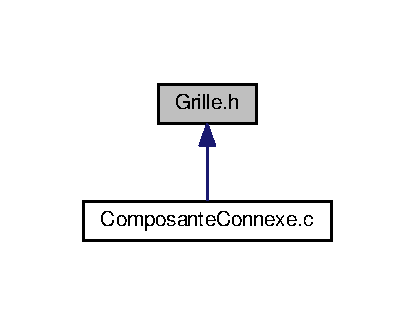
\includegraphics[width=199pt]{_grille_8h__dep__incl}
\end{center}
\end{figure}
\subsection*{Typedefs}
\begin{DoxyCompactItemize}
\item 
typedef struct \hyperlink{structt__case}{t\+\_\+case} \hyperlink{_grille_8h_adca0b8649254211841dc79ed6c528a86}{Case}
\end{DoxyCompactItemize}
\subsection*{Enumerations}
\begin{DoxyCompactItemize}
\item 
enum \hyperlink{_grille_8h_aa304d0ca681f782b1d7735da33037dd7}{Couleur} \{ \\*
\hyperlink{_grille_8c_aa304d0ca681f782b1d7735da33037dd7a3f2a77ecd272aa6d6b5902faa5e5fc68}{B}, 
\hyperlink{_grille_8c_aa304d0ca681f782b1d7735da33037dd7a28f41f1144eee94834387e9a6a088bc1}{V}, 
\hyperlink{_grille_8c_aa304d0ca681f782b1d7735da33037dd7a1784b1a3d7cbd43c45ff82c72d05e4ae}{R}, 
\hyperlink{_grille_8c_aa304d0ca681f782b1d7735da33037dd7a03605500b0c55f3d95874e8edfcf4e30}{J}, 
\\*
\hyperlink{_grille_8c_aa304d0ca681f782b1d7735da33037dd7a51ca6c63d97347ee58cc7da59ab6994b}{M}, 
\hyperlink{_grille_8c_aa304d0ca681f782b1d7735da33037dd7a2fe993340f6abb2234e543cd427df70b}{G}, 
\hyperlink{_grille_8h_aa304d0ca681f782b1d7735da33037dd7a3f2a77ecd272aa6d6b5902faa5e5fc68}{B}, 
\hyperlink{_grille_8h_aa304d0ca681f782b1d7735da33037dd7a28f41f1144eee94834387e9a6a088bc1}{V}, 
\\*
\hyperlink{_grille_8h_aa304d0ca681f782b1d7735da33037dd7a1784b1a3d7cbd43c45ff82c72d05e4ae}{R}, 
\hyperlink{_grille_8h_aa304d0ca681f782b1d7735da33037dd7a03605500b0c55f3d95874e8edfcf4e30}{J}, 
\hyperlink{_grille_8h_aa304d0ca681f782b1d7735da33037dd7a51ca6c63d97347ee58cc7da59ab6994b}{M}, 
\hyperlink{_grille_8h_aa304d0ca681f782b1d7735da33037dd7a2fe993340f6abb2234e543cd427df70b}{G}
 \}
\end{DoxyCompactItemize}
\subsection*{Functions}
\begin{DoxyCompactItemize}
\item 
int \hyperlink{_grille_8h_a802e561ca78785bfb07308847f57decc}{get\+X\+Case} (\hyperlink{_grille_8h_adca0b8649254211841dc79ed6c528a86}{Case} test)
\begin{DoxyCompactList}\small\item\em Récupère l\textquotesingle{}abscisse de la case considérée. \end{DoxyCompactList}\item 
int \hyperlink{_grille_8h_acfff6837eafd46f5269db9399503ae0c}{get\+Y\+Case} (\hyperlink{_grille_8h_adca0b8649254211841dc79ed6c528a86}{Case} test)
\begin{DoxyCompactList}\small\item\em Récupère l\textquotesingle{}ordonnée de la case considérée. \end{DoxyCompactList}\item 
int \hyperlink{_grille_8h_a1f67bc9aaa3d2b2e18bc56cbd64e9db4}{get\+Couleur\+Case} (\hyperlink{_grille_8h_adca0b8649254211841dc79ed6c528a86}{Case} test)
\begin{DoxyCompactList}\small\item\em Récupère la couleur de la case considérée. \end{DoxyCompactList}\item 
void \hyperlink{_grille_8h_afa2e284e68787b2997383a31eb764b97}{set\+Couleur} (\hyperlink{_grille_8h_adca0b8649254211841dc79ed6c528a86}{Case} $\ast$test, \hyperlink{_grille_8c_aa304d0ca681f782b1d7735da33037dd7}{Couleur} c)
\begin{DoxyCompactList}\small\item\em Change la couleur de la case considérée par la couleur en paramètre. \end{DoxyCompactList}\item 
\hyperlink{_grille_8h_adca0b8649254211841dc79ed6c528a86}{Case} $\ast$$\ast$ \hyperlink{_grille_8h_a1b8be80378b6a5b3fca696f93d67e1a9}{tableau\+Vide} (int n)
\begin{DoxyCompactList}\small\item\em Initialise un tableau vide de taille n. \end{DoxyCompactList}\item 
void \hyperlink{_grille_8h_a63924a00bcf27e9d394076c4659ae55c}{liberation\+Grille} (\hyperlink{_grille_8h_adca0b8649254211841dc79ed6c528a86}{Case} $\ast$$\ast$tab, int taille)
\begin{DoxyCompactList}\small\item\em Libère l\textquotesingle{}espace mémoire occupé par la grille. \end{DoxyCompactList}\item 
\hyperlink{_grille_8c_aa304d0ca681f782b1d7735da33037dd7}{Couleur} $\ast$$\ast$ \hyperlink{_grille_8h_af90a8c5a6dfed19c42a57f0ca19daf81}{remplissage\+Aleatoire} (int n)
\begin{DoxyCompactList}\small\item\em Fonction de remplissage aléatoire du tableau. \end{DoxyCompactList}\item 
\hyperlink{_grille_8c_aa304d0ca681f782b1d7735da33037dd7}{Couleur} $\ast$$\ast$ \hyperlink{_grille_8h_afd85b7e73c3be3858db354ee7f802683}{remplissage\+Fichier} (char $\ast$text)
\begin{DoxyCompactList}\small\item\em Crée un tableau de couleur à partir d\textquotesingle{}un fichier. Le fichier doit contenir des chaines de caractères contenant un retour à la ligne au bout de chaque ligne. \end{DoxyCompactList}\end{DoxyCompactItemize}


\subsection{Typedef Documentation}
\index{Grille.\+h@{Grille.\+h}!Case@{Case}}
\index{Case@{Case}!Grille.\+h@{Grille.\+h}}
\subsubsection[{\texorpdfstring{Case}{Case}}]{\setlength{\rightskip}{0pt plus 5cm}typedef struct {\bf t\+\_\+case} {\bf Case}}\hypertarget{_grille_8h_adca0b8649254211841dc79ed6c528a86}{}\label{_grille_8h_adca0b8649254211841dc79ed6c528a86}


\subsection{Enumeration Type Documentation}
\index{Grille.\+h@{Grille.\+h}!Couleur@{Couleur}}
\index{Couleur@{Couleur}!Grille.\+h@{Grille.\+h}}
\subsubsection[{\texorpdfstring{Couleur}{Couleur}}]{\setlength{\rightskip}{0pt plus 5cm}enum {\bf Couleur}}\hypertarget{_grille_8h_aa304d0ca681f782b1d7735da33037dd7}{}\label{_grille_8h_aa304d0ca681f782b1d7735da33037dd7}
\begin{Desc}
\item[Enumerator]\par
\begin{description}
\index{B@{B}!Grille.\+h@{Grille.\+h}}\index{Grille.\+h@{Grille.\+h}!B@{B}}\item[{\em 
B\hypertarget{_grille_8h_aa304d0ca681f782b1d7735da33037dd7a3f2a77ecd272aa6d6b5902faa5e5fc68}{}\label{_grille_8h_aa304d0ca681f782b1d7735da33037dd7a3f2a77ecd272aa6d6b5902faa5e5fc68}
}]\index{V@{V}!Grille.\+h@{Grille.\+h}}\index{Grille.\+h@{Grille.\+h}!V@{V}}\item[{\em 
V\hypertarget{_grille_8h_aa304d0ca681f782b1d7735da33037dd7a28f41f1144eee94834387e9a6a088bc1}{}\label{_grille_8h_aa304d0ca681f782b1d7735da33037dd7a28f41f1144eee94834387e9a6a088bc1}
}]\index{R@{R}!Grille.\+h@{Grille.\+h}}\index{Grille.\+h@{Grille.\+h}!R@{R}}\item[{\em 
R\hypertarget{_grille_8h_aa304d0ca681f782b1d7735da33037dd7a1784b1a3d7cbd43c45ff82c72d05e4ae}{}\label{_grille_8h_aa304d0ca681f782b1d7735da33037dd7a1784b1a3d7cbd43c45ff82c72d05e4ae}
}]\index{J@{J}!Grille.\+h@{Grille.\+h}}\index{Grille.\+h@{Grille.\+h}!J@{J}}\item[{\em 
J\hypertarget{_grille_8h_aa304d0ca681f782b1d7735da33037dd7a03605500b0c55f3d95874e8edfcf4e30}{}\label{_grille_8h_aa304d0ca681f782b1d7735da33037dd7a03605500b0c55f3d95874e8edfcf4e30}
}]\index{M@{M}!Grille.\+h@{Grille.\+h}}\index{Grille.\+h@{Grille.\+h}!M@{M}}\item[{\em 
M\hypertarget{_grille_8h_aa304d0ca681f782b1d7735da33037dd7a51ca6c63d97347ee58cc7da59ab6994b}{}\label{_grille_8h_aa304d0ca681f782b1d7735da33037dd7a51ca6c63d97347ee58cc7da59ab6994b}
}]\index{G@{G}!Grille.\+h@{Grille.\+h}}\index{Grille.\+h@{Grille.\+h}!G@{G}}\item[{\em 
G\hypertarget{_grille_8h_aa304d0ca681f782b1d7735da33037dd7a2fe993340f6abb2234e543cd427df70b}{}\label{_grille_8h_aa304d0ca681f782b1d7735da33037dd7a2fe993340f6abb2234e543cd427df70b}
}]\index{B@{B}!Grille.\+h@{Grille.\+h}}\index{Grille.\+h@{Grille.\+h}!B@{B}}\item[{\em 
B\hypertarget{_grille_8h_aa304d0ca681f782b1d7735da33037dd7a3f2a77ecd272aa6d6b5902faa5e5fc68}{}\label{_grille_8h_aa304d0ca681f782b1d7735da33037dd7a3f2a77ecd272aa6d6b5902faa5e5fc68}
}]\index{V@{V}!Grille.\+h@{Grille.\+h}}\index{Grille.\+h@{Grille.\+h}!V@{V}}\item[{\em 
V\hypertarget{_grille_8h_aa304d0ca681f782b1d7735da33037dd7a28f41f1144eee94834387e9a6a088bc1}{}\label{_grille_8h_aa304d0ca681f782b1d7735da33037dd7a28f41f1144eee94834387e9a6a088bc1}
}]\index{R@{R}!Grille.\+h@{Grille.\+h}}\index{Grille.\+h@{Grille.\+h}!R@{R}}\item[{\em 
R\hypertarget{_grille_8h_aa304d0ca681f782b1d7735da33037dd7a1784b1a3d7cbd43c45ff82c72d05e4ae}{}\label{_grille_8h_aa304d0ca681f782b1d7735da33037dd7a1784b1a3d7cbd43c45ff82c72d05e4ae}
}]\index{J@{J}!Grille.\+h@{Grille.\+h}}\index{Grille.\+h@{Grille.\+h}!J@{J}}\item[{\em 
J\hypertarget{_grille_8h_aa304d0ca681f782b1d7735da33037dd7a03605500b0c55f3d95874e8edfcf4e30}{}\label{_grille_8h_aa304d0ca681f782b1d7735da33037dd7a03605500b0c55f3d95874e8edfcf4e30}
}]\index{M@{M}!Grille.\+h@{Grille.\+h}}\index{Grille.\+h@{Grille.\+h}!M@{M}}\item[{\em 
M\hypertarget{_grille_8h_aa304d0ca681f782b1d7735da33037dd7a51ca6c63d97347ee58cc7da59ab6994b}{}\label{_grille_8h_aa304d0ca681f782b1d7735da33037dd7a51ca6c63d97347ee58cc7da59ab6994b}
}]\index{G@{G}!Grille.\+h@{Grille.\+h}}\index{Grille.\+h@{Grille.\+h}!G@{G}}\item[{\em 
G\hypertarget{_grille_8h_aa304d0ca681f782b1d7735da33037dd7a2fe993340f6abb2234e543cd427df70b}{}\label{_grille_8h_aa304d0ca681f782b1d7735da33037dd7a2fe993340f6abb2234e543cd427df70b}
}]\end{description}
\end{Desc}


\subsection{Function Documentation}
\index{Grille.\+h@{Grille.\+h}!get\+Couleur\+Case@{get\+Couleur\+Case}}
\index{get\+Couleur\+Case@{get\+Couleur\+Case}!Grille.\+h@{Grille.\+h}}
\subsubsection[{\texorpdfstring{get\+Couleur\+Case(\+Case test)}{getCouleurCase(Case test)}}]{\setlength{\rightskip}{0pt plus 5cm}int get\+Couleur\+Case (
\begin{DoxyParamCaption}
\item[{{\bf Case}}]{test}
\end{DoxyParamCaption}
)}\hypertarget{_grille_8h_a1f67bc9aaa3d2b2e18bc56cbd64e9db4}{}\label{_grille_8h_a1f67bc9aaa3d2b2e18bc56cbd64e9db4}


Récupère la couleur de la case considérée. 

\begin{DoxyAuthor}{Author}
Hélène Tran 
\end{DoxyAuthor}
\index{Grille.\+h@{Grille.\+h}!get\+X\+Case@{get\+X\+Case}}
\index{get\+X\+Case@{get\+X\+Case}!Grille.\+h@{Grille.\+h}}
\subsubsection[{\texorpdfstring{get\+X\+Case(\+Case test)}{getXCase(Case test)}}]{\setlength{\rightskip}{0pt plus 5cm}int get\+X\+Case (
\begin{DoxyParamCaption}
\item[{{\bf Case}}]{test}
\end{DoxyParamCaption}
)}\hypertarget{_grille_8h_a802e561ca78785bfb07308847f57decc}{}\label{_grille_8h_a802e561ca78785bfb07308847f57decc}


Récupère l\textquotesingle{}abscisse de la case considérée. 

\begin{DoxyAuthor}{Author}
Hélène Tran 
\end{DoxyAuthor}
\index{Grille.\+h@{Grille.\+h}!get\+Y\+Case@{get\+Y\+Case}}
\index{get\+Y\+Case@{get\+Y\+Case}!Grille.\+h@{Grille.\+h}}
\subsubsection[{\texorpdfstring{get\+Y\+Case(\+Case test)}{getYCase(Case test)}}]{\setlength{\rightskip}{0pt plus 5cm}int get\+Y\+Case (
\begin{DoxyParamCaption}
\item[{{\bf Case}}]{test}
\end{DoxyParamCaption}
)}\hypertarget{_grille_8h_acfff6837eafd46f5269db9399503ae0c}{}\label{_grille_8h_acfff6837eafd46f5269db9399503ae0c}


Récupère l\textquotesingle{}ordonnée de la case considérée. 

\begin{DoxyAuthor}{Author}
Hélène Tran 
\end{DoxyAuthor}
\index{Grille.\+h@{Grille.\+h}!liberation\+Grille@{liberation\+Grille}}
\index{liberation\+Grille@{liberation\+Grille}!Grille.\+h@{Grille.\+h}}
\subsubsection[{\texorpdfstring{liberation\+Grille(\+Case $\ast$$\ast$tab, int taille)}{liberationGrille(Case **tab, int taille)}}]{\setlength{\rightskip}{0pt plus 5cm}void liberation\+Grille (
\begin{DoxyParamCaption}
\item[{{\bf Case} $\ast$$\ast$}]{tab, }
\item[{int}]{taille}
\end{DoxyParamCaption}
)}\hypertarget{_grille_8h_a63924a00bcf27e9d394076c4659ae55c}{}\label{_grille_8h_a63924a00bcf27e9d394076c4659ae55c}


Libère l\textquotesingle{}espace mémoire occupé par la grille. 

\begin{DoxyAuthor}{Author}
Hélène Tran 
\end{DoxyAuthor}
\index{Grille.\+h@{Grille.\+h}!remplissage\+Aleatoire@{remplissage\+Aleatoire}}
\index{remplissage\+Aleatoire@{remplissage\+Aleatoire}!Grille.\+h@{Grille.\+h}}
\subsubsection[{\texorpdfstring{remplissage\+Aleatoire(int n)}{remplissageAleatoire(int n)}}]{\setlength{\rightskip}{0pt plus 5cm}{\bf Couleur}$\ast$$\ast$ remplissage\+Aleatoire (
\begin{DoxyParamCaption}
\item[{int}]{n}
\end{DoxyParamCaption}
)}\hypertarget{_grille_8h_af90a8c5a6dfed19c42a57f0ca19daf81}{}\label{_grille_8h_af90a8c5a6dfed19c42a57f0ca19daf81}


Fonction de remplissage aléatoire du tableau. 

\begin{DoxyAuthor}{Author}
Hélène Tran 
\end{DoxyAuthor}
\index{Grille.\+h@{Grille.\+h}!remplissage\+Fichier@{remplissage\+Fichier}}
\index{remplissage\+Fichier@{remplissage\+Fichier}!Grille.\+h@{Grille.\+h}}
\subsubsection[{\texorpdfstring{remplissage\+Fichier(char $\ast$text)}{remplissageFichier(char *text)}}]{\setlength{\rightskip}{0pt plus 5cm}{\bf Couleur}$\ast$$\ast$ remplissage\+Fichier (
\begin{DoxyParamCaption}
\item[{char $\ast$}]{text}
\end{DoxyParamCaption}
)}\hypertarget{_grille_8h_afd85b7e73c3be3858db354ee7f802683}{}\label{_grille_8h_afd85b7e73c3be3858db354ee7f802683}


Crée un tableau de couleur à partir d\textquotesingle{}un fichier. Le fichier doit contenir des chaines de caractères contenant un retour à la ligne au bout de chaque ligne. 

\begin{DoxyAuthor}{Author}
Hélène Tran 
\end{DoxyAuthor}
\index{Grille.\+h@{Grille.\+h}!set\+Couleur@{set\+Couleur}}
\index{set\+Couleur@{set\+Couleur}!Grille.\+h@{Grille.\+h}}
\subsubsection[{\texorpdfstring{set\+Couleur(\+Case $\ast$test, Couleur c)}{setCouleur(Case *test, Couleur c)}}]{\setlength{\rightskip}{0pt plus 5cm}void set\+Couleur (
\begin{DoxyParamCaption}
\item[{{\bf Case} $\ast$}]{test, }
\item[{{\bf Couleur}}]{c}
\end{DoxyParamCaption}
)}\hypertarget{_grille_8h_afa2e284e68787b2997383a31eb764b97}{}\label{_grille_8h_afa2e284e68787b2997383a31eb764b97}


Change la couleur de la case considérée par la couleur en paramètre. 

\begin{DoxyAuthor}{Author}
Hélène Tran 
\end{DoxyAuthor}
\index{Grille.\+h@{Grille.\+h}!tableau\+Vide@{tableau\+Vide}}
\index{tableau\+Vide@{tableau\+Vide}!Grille.\+h@{Grille.\+h}}
\subsubsection[{\texorpdfstring{tableau\+Vide(int n)}{tableauVide(int n)}}]{\setlength{\rightskip}{0pt plus 5cm}{\bf Case}$\ast$$\ast$ tableau\+Vide (
\begin{DoxyParamCaption}
\item[{int}]{n}
\end{DoxyParamCaption}
)}\hypertarget{_grille_8h_a1b8be80378b6a5b3fca696f93d67e1a9}{}\label{_grille_8h_a1b8be80378b6a5b3fca696f93d67e1a9}


Initialise un tableau vide de taille n. 

\begin{DoxyAuthor}{Author}
Hélène Tran 
\end{DoxyAuthor}

\hypertarget{_liste_composante_connexe_8c}{}\section{Liste\+Composante\+Connexe.\+c File Reference}
\label{_liste_composante_connexe_8c}\index{Liste\+Composante\+Connexe.\+c@{Liste\+Composante\+Connexe.\+c}}
{\ttfamily \#include \char`\"{}Liste\+Composante\+Connexe.\+h\char`\"{}}\\*
{\ttfamily \#include \char`\"{}Composante\+Connexe.\+h\char`\"{}}\\*
Include dependency graph for Liste\+Composante\+Connexe.\+c\+:\nopagebreak
\begin{figure}[H]
\begin{center}
\leavevmode
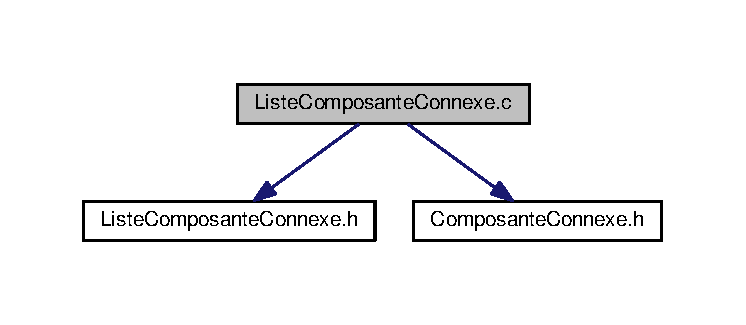
\includegraphics[width=350pt]{_liste_composante_connexe_8c__incl}
\end{center}
\end{figure}
\subsection*{Data Structures}
\begin{DoxyCompactItemize}
\item 
struct \hyperlink{structt___liste_composante_connexe}{t\+\_\+\+Liste\+Composante\+Connexe}
\end{DoxyCompactItemize}
\subsection*{Functions}
\begin{DoxyCompactItemize}
\item 
struct \hyperlink{structt___liste_composante_connexe}{t\+\_\+\+Liste\+Composante\+Connexe} \hyperlink{_liste_composante_connexe_8c_a23dc4d3f78ab71a19f01917d04955e41}{init\+Liste\+Composante\+Connexe} (void)
\item 
int \hyperlink{_liste_composante_connexe_8c_a8446c463a431710d16dd71816144f6ad}{est\+Vide\+Liste\+Composante\+Connexe} (\hyperlink{_liste_composante_connexe_8h_a8002dafd0bddf66157ac8cf6e811e4e7}{Liste\+Composante\+Connexe} l)
\item 
\hyperlink{struct_composante_connexe}{Composante\+Connexe} \hyperlink{_liste_composante_connexe_8c_a5033738216986309fd2b77e05c2a1f2e}{get\+Valeur\+Liste\+Composante\+Connexe} (\hyperlink{_liste_composante_connexe_8h_a8002dafd0bddf66157ac8cf6e811e4e7}{Liste\+Composante\+Connexe} l)
\item 
\hyperlink{_liste_composante_connexe_8h_a8002dafd0bddf66157ac8cf6e811e4e7}{Liste\+Composante\+Connexe} \hyperlink{_liste_composante_connexe_8c_a19c4681d03114d04954be943dcfa55fe}{get\+Suivant\+Liste\+Composante\+Connexe} (\hyperlink{_liste_composante_connexe_8h_a8002dafd0bddf66157ac8cf6e811e4e7}{Liste\+Composante\+Connexe} l)
\item 
\hyperlink{_liste_composante_connexe_8h_a8002dafd0bddf66157ac8cf6e811e4e7}{Liste\+Composante\+Connexe} \hyperlink{_liste_composante_connexe_8c_a74138fbec59760f5e873956ca350c9f3}{constructeur\+Liste\+Composante\+Connexe} (\hyperlink{_liste_composante_connexe_8h_a8002dafd0bddf66157ac8cf6e811e4e7}{Liste\+Composante\+Connexe} l, \hyperlink{struct_composante_connexe}{Composante\+Connexe} c)
\item 
void \hyperlink{_liste_composante_connexe_8c_a7672da5523783bac548dcbb99992dc67}{destructeur\+Liste\+Composante\+Connexe} (\hyperlink{_liste_composante_connexe_8h_a8002dafd0bddf66157ac8cf6e811e4e7}{Liste\+Composante\+Connexe} l)
\item 
int \hyperlink{_liste_composante_connexe_8c_a9c2fce1c8342c0a7c6fbcb378f9dace8}{longeur\+Liste\+Composante\+Connexe} (\hyperlink{_liste_composante_connexe_8h_a8002dafd0bddf66157ac8cf6e811e4e7}{Liste\+Composante\+Connexe} l)
\item 
int \hyperlink{_liste_composante_connexe_8c_ac0758234563b5891d7302d2fca6188c0}{test\+Victoire} (\hyperlink{_liste_composante_connexe_8h_a8002dafd0bddf66157ac8cf6e811e4e7}{Liste\+Composante\+Connexe} l)
\item 
\hyperlink{struct_composante_connexe}{Composante\+Connexe} $\ast$ \hyperlink{_liste_composante_connexe_8c_a30f5132aad814efb80e12b7ce53bdab4}{recherche\+Element\+Liste\+Composante\+Connexe} (\hyperlink{_liste_composante_connexe_8h_a8002dafd0bddf66157ac8cf6e811e4e7}{Liste\+Composante\+Connexe} l, \hyperlink{struct_composante_connexe}{Composante\+Connexe} element)
\item 
void \hyperlink{_liste_composante_connexe_8c_a139cf52901c50eb1482396787404bdd8}{supprime\+Element\+Liste\+Composante\+Connexe} (\hyperlink{_liste_composante_connexe_8h_a8002dafd0bddf66157ac8cf6e811e4e7}{Liste\+Composante\+Connexe} $\ast$l, \hyperlink{struct_composante_connexe}{Composante\+Connexe} element)
\end{DoxyCompactItemize}
\subsection*{Variables}
\begin{DoxyCompactItemize}
\item 
\hyperlink{struct_composante_connexe}{Composante\+Connexe} \hyperlink{_liste_composante_connexe_8c_a014090efb1c03d5f1036780b1390bc68}{composantec}
\item 
struct \hyperlink{_liste_composante_connexe_8h_a8002dafd0bddf66157ac8cf6e811e4e7}{Liste\+Composante\+Connexe} $\ast$ \hyperlink{_liste_composante_connexe_8c_a1de430f247ea74c5770d3fdfcc58d98a}{suivant}
\end{DoxyCompactItemize}


\subsection{Function Documentation}
\index{Liste\+Composante\+Connexe.\+c@{Liste\+Composante\+Connexe.\+c}!constructeur\+Liste\+Composante\+Connexe@{constructeur\+Liste\+Composante\+Connexe}}
\index{constructeur\+Liste\+Composante\+Connexe@{constructeur\+Liste\+Composante\+Connexe}!Liste\+Composante\+Connexe.\+c@{Liste\+Composante\+Connexe.\+c}}
\subsubsection[{\texorpdfstring{constructeur\+Liste\+Composante\+Connexe(\+Liste\+Composante\+Connexe l, Composante\+Connexe c)}{constructeurListeComposanteConnexe(ListeComposanteConnexe l, ComposanteConnexe c)}}]{\setlength{\rightskip}{0pt plus 5cm}{\bf Liste\+Composante\+Connexe} constructeur\+Liste\+Composante\+Connexe (
\begin{DoxyParamCaption}
\item[{{\bf Liste\+Composante\+Connexe}}]{l, }
\item[{{\bf Composante\+Connexe}}]{c}
\end{DoxyParamCaption}
)}\hypertarget{_liste_composante_connexe_8c_a74138fbec59760f5e873956ca350c9f3}{}\label{_liste_composante_connexe_8c_a74138fbec59760f5e873956ca350c9f3}
\index{Liste\+Composante\+Connexe.\+c@{Liste\+Composante\+Connexe.\+c}!destructeur\+Liste\+Composante\+Connexe@{destructeur\+Liste\+Composante\+Connexe}}
\index{destructeur\+Liste\+Composante\+Connexe@{destructeur\+Liste\+Composante\+Connexe}!Liste\+Composante\+Connexe.\+c@{Liste\+Composante\+Connexe.\+c}}
\subsubsection[{\texorpdfstring{destructeur\+Liste\+Composante\+Connexe(\+Liste\+Composante\+Connexe l)}{destructeurListeComposanteConnexe(ListeComposanteConnexe l)}}]{\setlength{\rightskip}{0pt plus 5cm}void destructeur\+Liste\+Composante\+Connexe (
\begin{DoxyParamCaption}
\item[{{\bf Liste\+Composante\+Connexe}}]{l}
\end{DoxyParamCaption}
)}\hypertarget{_liste_composante_connexe_8c_a7672da5523783bac548dcbb99992dc67}{}\label{_liste_composante_connexe_8c_a7672da5523783bac548dcbb99992dc67}
\index{Liste\+Composante\+Connexe.\+c@{Liste\+Composante\+Connexe.\+c}!est\+Vide\+Liste\+Composante\+Connexe@{est\+Vide\+Liste\+Composante\+Connexe}}
\index{est\+Vide\+Liste\+Composante\+Connexe@{est\+Vide\+Liste\+Composante\+Connexe}!Liste\+Composante\+Connexe.\+c@{Liste\+Composante\+Connexe.\+c}}
\subsubsection[{\texorpdfstring{est\+Vide\+Liste\+Composante\+Connexe(\+Liste\+Composante\+Connexe l)}{estVideListeComposanteConnexe(ListeComposanteConnexe l)}}]{\setlength{\rightskip}{0pt plus 5cm}int est\+Vide\+Liste\+Composante\+Connexe (
\begin{DoxyParamCaption}
\item[{{\bf Liste\+Composante\+Connexe}}]{l}
\end{DoxyParamCaption}
)}\hypertarget{_liste_composante_connexe_8c_a8446c463a431710d16dd71816144f6ad}{}\label{_liste_composante_connexe_8c_a8446c463a431710d16dd71816144f6ad}
\index{Liste\+Composante\+Connexe.\+c@{Liste\+Composante\+Connexe.\+c}!get\+Suivant\+Liste\+Composante\+Connexe@{get\+Suivant\+Liste\+Composante\+Connexe}}
\index{get\+Suivant\+Liste\+Composante\+Connexe@{get\+Suivant\+Liste\+Composante\+Connexe}!Liste\+Composante\+Connexe.\+c@{Liste\+Composante\+Connexe.\+c}}
\subsubsection[{\texorpdfstring{get\+Suivant\+Liste\+Composante\+Connexe(\+Liste\+Composante\+Connexe l)}{getSuivantListeComposanteConnexe(ListeComposanteConnexe l)}}]{\setlength{\rightskip}{0pt plus 5cm}{\bf Liste\+Composante\+Connexe} get\+Suivant\+Liste\+Composante\+Connexe (
\begin{DoxyParamCaption}
\item[{{\bf Liste\+Composante\+Connexe}}]{l}
\end{DoxyParamCaption}
)}\hypertarget{_liste_composante_connexe_8c_a19c4681d03114d04954be943dcfa55fe}{}\label{_liste_composante_connexe_8c_a19c4681d03114d04954be943dcfa55fe}
\index{Liste\+Composante\+Connexe.\+c@{Liste\+Composante\+Connexe.\+c}!get\+Valeur\+Liste\+Composante\+Connexe@{get\+Valeur\+Liste\+Composante\+Connexe}}
\index{get\+Valeur\+Liste\+Composante\+Connexe@{get\+Valeur\+Liste\+Composante\+Connexe}!Liste\+Composante\+Connexe.\+c@{Liste\+Composante\+Connexe.\+c}}
\subsubsection[{\texorpdfstring{get\+Valeur\+Liste\+Composante\+Connexe(\+Liste\+Composante\+Connexe l)}{getValeurListeComposanteConnexe(ListeComposanteConnexe l)}}]{\setlength{\rightskip}{0pt plus 5cm}{\bf Composante\+Connexe} get\+Valeur\+Liste\+Composante\+Connexe (
\begin{DoxyParamCaption}
\item[{{\bf Liste\+Composante\+Connexe}}]{l}
\end{DoxyParamCaption}
)}\hypertarget{_liste_composante_connexe_8c_a5033738216986309fd2b77e05c2a1f2e}{}\label{_liste_composante_connexe_8c_a5033738216986309fd2b77e05c2a1f2e}
\index{Liste\+Composante\+Connexe.\+c@{Liste\+Composante\+Connexe.\+c}!init\+Liste\+Composante\+Connexe@{init\+Liste\+Composante\+Connexe}}
\index{init\+Liste\+Composante\+Connexe@{init\+Liste\+Composante\+Connexe}!Liste\+Composante\+Connexe.\+c@{Liste\+Composante\+Connexe.\+c}}
\subsubsection[{\texorpdfstring{init\+Liste\+Composante\+Connexe(void)}{initListeComposanteConnexe(void)}}]{\setlength{\rightskip}{0pt plus 5cm}struct {\bf t\+\_\+\+Liste\+Composante\+Connexe} init\+Liste\+Composante\+Connexe (
\begin{DoxyParamCaption}
\item[{void}]{}
\end{DoxyParamCaption}
)}\hypertarget{_liste_composante_connexe_8c_a23dc4d3f78ab71a19f01917d04955e41}{}\label{_liste_composante_connexe_8c_a23dc4d3f78ab71a19f01917d04955e41}
\index{Liste\+Composante\+Connexe.\+c@{Liste\+Composante\+Connexe.\+c}!longeur\+Liste\+Composante\+Connexe@{longeur\+Liste\+Composante\+Connexe}}
\index{longeur\+Liste\+Composante\+Connexe@{longeur\+Liste\+Composante\+Connexe}!Liste\+Composante\+Connexe.\+c@{Liste\+Composante\+Connexe.\+c}}
\subsubsection[{\texorpdfstring{longeur\+Liste\+Composante\+Connexe(\+Liste\+Composante\+Connexe l)}{longeurListeComposanteConnexe(ListeComposanteConnexe l)}}]{\setlength{\rightskip}{0pt plus 5cm}int longeur\+Liste\+Composante\+Connexe (
\begin{DoxyParamCaption}
\item[{{\bf Liste\+Composante\+Connexe}}]{l}
\end{DoxyParamCaption}
)}\hypertarget{_liste_composante_connexe_8c_a9c2fce1c8342c0a7c6fbcb378f9dace8}{}\label{_liste_composante_connexe_8c_a9c2fce1c8342c0a7c6fbcb378f9dace8}
\index{Liste\+Composante\+Connexe.\+c@{Liste\+Composante\+Connexe.\+c}!recherche\+Element\+Liste\+Composante\+Connexe@{recherche\+Element\+Liste\+Composante\+Connexe}}
\index{recherche\+Element\+Liste\+Composante\+Connexe@{recherche\+Element\+Liste\+Composante\+Connexe}!Liste\+Composante\+Connexe.\+c@{Liste\+Composante\+Connexe.\+c}}
\subsubsection[{\texorpdfstring{recherche\+Element\+Liste\+Composante\+Connexe(\+Liste\+Composante\+Connexe l, Composante\+Connexe element)}{rechercheElementListeComposanteConnexe(ListeComposanteConnexe l, ComposanteConnexe element)}}]{\setlength{\rightskip}{0pt plus 5cm}{\bf Composante\+Connexe}$\ast$ recherche\+Element\+Liste\+Composante\+Connexe (
\begin{DoxyParamCaption}
\item[{{\bf Liste\+Composante\+Connexe}}]{l, }
\item[{{\bf Composante\+Connexe}}]{element}
\end{DoxyParamCaption}
)}\hypertarget{_liste_composante_connexe_8c_a30f5132aad814efb80e12b7ce53bdab4}{}\label{_liste_composante_connexe_8c_a30f5132aad814efb80e12b7ce53bdab4}
\index{Liste\+Composante\+Connexe.\+c@{Liste\+Composante\+Connexe.\+c}!supprime\+Element\+Liste\+Composante\+Connexe@{supprime\+Element\+Liste\+Composante\+Connexe}}
\index{supprime\+Element\+Liste\+Composante\+Connexe@{supprime\+Element\+Liste\+Composante\+Connexe}!Liste\+Composante\+Connexe.\+c@{Liste\+Composante\+Connexe.\+c}}
\subsubsection[{\texorpdfstring{supprime\+Element\+Liste\+Composante\+Connexe(\+Liste\+Composante\+Connexe $\ast$l, Composante\+Connexe element)}{supprimeElementListeComposanteConnexe(ListeComposanteConnexe *l, ComposanteConnexe element)}}]{\setlength{\rightskip}{0pt plus 5cm}void supprime\+Element\+Liste\+Composante\+Connexe (
\begin{DoxyParamCaption}
\item[{{\bf Liste\+Composante\+Connexe} $\ast$}]{l, }
\item[{{\bf Composante\+Connexe}}]{element}
\end{DoxyParamCaption}
)}\hypertarget{_liste_composante_connexe_8c_a139cf52901c50eb1482396787404bdd8}{}\label{_liste_composante_connexe_8c_a139cf52901c50eb1482396787404bdd8}
\index{Liste\+Composante\+Connexe.\+c@{Liste\+Composante\+Connexe.\+c}!test\+Victoire@{test\+Victoire}}
\index{test\+Victoire@{test\+Victoire}!Liste\+Composante\+Connexe.\+c@{Liste\+Composante\+Connexe.\+c}}
\subsubsection[{\texorpdfstring{test\+Victoire(\+Liste\+Composante\+Connexe l)}{testVictoire(ListeComposanteConnexe l)}}]{\setlength{\rightskip}{0pt plus 5cm}int test\+Victoire (
\begin{DoxyParamCaption}
\item[{{\bf Liste\+Composante\+Connexe}}]{l}
\end{DoxyParamCaption}
)}\hypertarget{_liste_composante_connexe_8c_ac0758234563b5891d7302d2fca6188c0}{}\label{_liste_composante_connexe_8c_ac0758234563b5891d7302d2fca6188c0}


\subsection{Variable Documentation}
\index{Liste\+Composante\+Connexe.\+c@{Liste\+Composante\+Connexe.\+c}!composantec@{composantec}}
\index{composantec@{composantec}!Liste\+Composante\+Connexe.\+c@{Liste\+Composante\+Connexe.\+c}}
\subsubsection[{\texorpdfstring{composantec}{composantec}}]{\setlength{\rightskip}{0pt plus 5cm}{\bf Composante\+Connexe} composantec}\hypertarget{_liste_composante_connexe_8c_a014090efb1c03d5f1036780b1390bc68}{}\label{_liste_composante_connexe_8c_a014090efb1c03d5f1036780b1390bc68}
\index{Liste\+Composante\+Connexe.\+c@{Liste\+Composante\+Connexe.\+c}!suivant@{suivant}}
\index{suivant@{suivant}!Liste\+Composante\+Connexe.\+c@{Liste\+Composante\+Connexe.\+c}}
\subsubsection[{\texorpdfstring{suivant}{suivant}}]{\setlength{\rightskip}{0pt plus 5cm}struct {\bf Liste\+Composante\+Connexe}$\ast$ suivant}\hypertarget{_liste_composante_connexe_8c_a1de430f247ea74c5770d3fdfcc58d98a}{}\label{_liste_composante_connexe_8c_a1de430f247ea74c5770d3fdfcc58d98a}

\hypertarget{_liste_composante_connexe_8h}{}\section{Liste\+Composante\+Connexe.\+h File Reference}
\label{_liste_composante_connexe_8h}\index{Liste\+Composante\+Connexe.\+h@{Liste\+Composante\+Connexe.\+h}}
This graph shows which files directly or indirectly include this file\+:\nopagebreak
\begin{figure}[H]
\begin{center}
\leavevmode
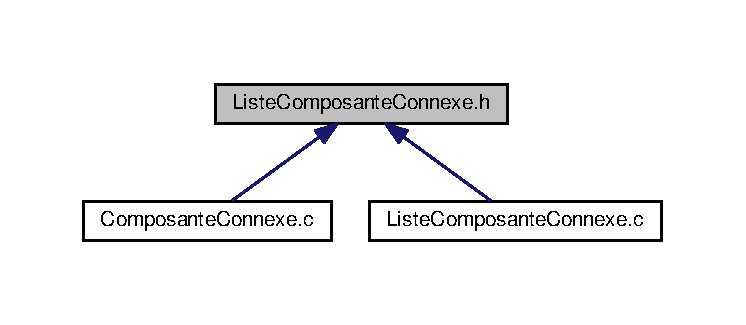
\includegraphics[width=350pt]{_liste_composante_connexe_8h__dep__incl}
\end{center}
\end{figure}
\subsection*{Typedefs}
\begin{DoxyCompactItemize}
\item 
typedef struct \hyperlink{structt___liste_composante_connexe}{t\+\_\+\+Liste\+Composante\+Connexe} \hyperlink{_liste_composante_connexe_8h_a5b62a8a95ba9e4fb45be39b0c77e96ca}{Cellule\+Composante\+Connexe}
\item 
typedef \hyperlink{_liste_composante_connexe_8h_a5b62a8a95ba9e4fb45be39b0c77e96ca}{Cellule\+Composante\+Connexe} $\ast$ \hyperlink{_liste_composante_connexe_8h_a8002dafd0bddf66157ac8cf6e811e4e7}{Liste\+Composante\+Connexe}
\end{DoxyCompactItemize}
\subsection*{Functions}
\begin{DoxyCompactItemize}
\item 
\hyperlink{_liste_composante_connexe_8h_a8002dafd0bddf66157ac8cf6e811e4e7}{Liste\+Composante\+Connexe} \hyperlink{_liste_composante_connexe_8h_a95d66715a101da0f5f315bc05074bc9f}{init\+Liste\+Composante\+Connexe} (void)
\item 
int \hyperlink{_liste_composante_connexe_8h_a8446c463a431710d16dd71816144f6ad}{est\+Vide\+Liste\+Composante\+Connexe} (\hyperlink{_liste_composante_connexe_8h_a8002dafd0bddf66157ac8cf6e811e4e7}{Liste\+Composante\+Connexe} l)
\item 
\hyperlink{_liste_composante_connexe_8h_a8002dafd0bddf66157ac8cf6e811e4e7}{Liste\+Composante\+Connexe} \hyperlink{_liste_composante_connexe_8h_a74138fbec59760f5e873956ca350c9f3}{constructeur\+Liste\+Composante\+Connexe} (\hyperlink{_liste_composante_connexe_8h_a8002dafd0bddf66157ac8cf6e811e4e7}{Liste\+Composante\+Connexe} l, \hyperlink{struct_composante_connexe}{Composante\+Connexe} c)
\item 
int \hyperlink{_liste_composante_connexe_8h_a9c2fce1c8342c0a7c6fbcb378f9dace8}{longeur\+Liste\+Composante\+Connexe} (\hyperlink{_liste_composante_connexe_8h_a8002dafd0bddf66157ac8cf6e811e4e7}{Liste\+Composante\+Connexe} l)
\item 
int \hyperlink{_liste_composante_connexe_8h_ac0758234563b5891d7302d2fca6188c0}{test\+Victoire} (\hyperlink{_liste_composante_connexe_8h_a8002dafd0bddf66157ac8cf6e811e4e7}{Liste\+Composante\+Connexe} l)
\item 
\hyperlink{struct_composante_connexe}{Composante\+Connexe} \hyperlink{_liste_composante_connexe_8h_a5033738216986309fd2b77e05c2a1f2e}{get\+Valeur\+Liste\+Composante\+Connexe} (\hyperlink{_liste_composante_connexe_8h_a8002dafd0bddf66157ac8cf6e811e4e7}{Liste\+Composante\+Connexe} l)
\item 
\hyperlink{_liste_composante_connexe_8h_a8002dafd0bddf66157ac8cf6e811e4e7}{Liste\+Composante\+Connexe} \hyperlink{_liste_composante_connexe_8h_a19c4681d03114d04954be943dcfa55fe}{get\+Suivant\+Liste\+Composante\+Connexe} (\hyperlink{_liste_composante_connexe_8h_a8002dafd0bddf66157ac8cf6e811e4e7}{Liste\+Composante\+Connexe} l)
\item 
void \hyperlink{_liste_composante_connexe_8h_a7672da5523783bac548dcbb99992dc67}{destructeur\+Liste\+Composante\+Connexe} (\hyperlink{_liste_composante_connexe_8h_a8002dafd0bddf66157ac8cf6e811e4e7}{Liste\+Composante\+Connexe} l)
\item 
\hyperlink{struct_composante_connexe}{Composante\+Connexe} $\ast$ \hyperlink{_liste_composante_connexe_8h_a30f5132aad814efb80e12b7ce53bdab4}{recherche\+Element\+Liste\+Composante\+Connexe} (\hyperlink{_liste_composante_connexe_8h_a8002dafd0bddf66157ac8cf6e811e4e7}{Liste\+Composante\+Connexe} l, \hyperlink{struct_composante_connexe}{Composante\+Connexe} element)
\item 
void \hyperlink{_liste_composante_connexe_8h_a139cf52901c50eb1482396787404bdd8}{supprime\+Element\+Liste\+Composante\+Connexe} (\hyperlink{_liste_composante_connexe_8h_a8002dafd0bddf66157ac8cf6e811e4e7}{Liste\+Composante\+Connexe} $\ast$l, \hyperlink{struct_composante_connexe}{Composante\+Connexe} element)
\end{DoxyCompactItemize}


\subsection{Typedef Documentation}
\index{Liste\+Composante\+Connexe.\+h@{Liste\+Composante\+Connexe.\+h}!Cellule\+Composante\+Connexe@{Cellule\+Composante\+Connexe}}
\index{Cellule\+Composante\+Connexe@{Cellule\+Composante\+Connexe}!Liste\+Composante\+Connexe.\+h@{Liste\+Composante\+Connexe.\+h}}
\subsubsection[{\texorpdfstring{Cellule\+Composante\+Connexe}{CelluleComposanteConnexe}}]{\setlength{\rightskip}{0pt plus 5cm}typedef struct {\bf t\+\_\+\+Liste\+Composante\+Connexe} {\bf Cellule\+Composante\+Connexe}}\hypertarget{_liste_composante_connexe_8h_a5b62a8a95ba9e4fb45be39b0c77e96ca}{}\label{_liste_composante_connexe_8h_a5b62a8a95ba9e4fb45be39b0c77e96ca}
\index{Liste\+Composante\+Connexe.\+h@{Liste\+Composante\+Connexe.\+h}!Liste\+Composante\+Connexe@{Liste\+Composante\+Connexe}}
\index{Liste\+Composante\+Connexe@{Liste\+Composante\+Connexe}!Liste\+Composante\+Connexe.\+h@{Liste\+Composante\+Connexe.\+h}}
\subsubsection[{\texorpdfstring{Liste\+Composante\+Connexe}{ListeComposanteConnexe}}]{\setlength{\rightskip}{0pt plus 5cm}typedef {\bf Cellule\+Composante\+Connexe}$\ast$ {\bf Liste\+Composante\+Connexe}}\hypertarget{_liste_composante_connexe_8h_a8002dafd0bddf66157ac8cf6e811e4e7}{}\label{_liste_composante_connexe_8h_a8002dafd0bddf66157ac8cf6e811e4e7}


\subsection{Function Documentation}
\index{Liste\+Composante\+Connexe.\+h@{Liste\+Composante\+Connexe.\+h}!constructeur\+Liste\+Composante\+Connexe@{constructeur\+Liste\+Composante\+Connexe}}
\index{constructeur\+Liste\+Composante\+Connexe@{constructeur\+Liste\+Composante\+Connexe}!Liste\+Composante\+Connexe.\+h@{Liste\+Composante\+Connexe.\+h}}
\subsubsection[{\texorpdfstring{constructeur\+Liste\+Composante\+Connexe(\+Liste\+Composante\+Connexe l, Composante\+Connexe c)}{constructeurListeComposanteConnexe(ListeComposanteConnexe l, ComposanteConnexe c)}}]{\setlength{\rightskip}{0pt plus 5cm}{\bf Liste\+Composante\+Connexe} constructeur\+Liste\+Composante\+Connexe (
\begin{DoxyParamCaption}
\item[{{\bf Liste\+Composante\+Connexe}}]{l, }
\item[{{\bf Composante\+Connexe}}]{c}
\end{DoxyParamCaption}
)}\hypertarget{_liste_composante_connexe_8h_a74138fbec59760f5e873956ca350c9f3}{}\label{_liste_composante_connexe_8h_a74138fbec59760f5e873956ca350c9f3}
\index{Liste\+Composante\+Connexe.\+h@{Liste\+Composante\+Connexe.\+h}!destructeur\+Liste\+Composante\+Connexe@{destructeur\+Liste\+Composante\+Connexe}}
\index{destructeur\+Liste\+Composante\+Connexe@{destructeur\+Liste\+Composante\+Connexe}!Liste\+Composante\+Connexe.\+h@{Liste\+Composante\+Connexe.\+h}}
\subsubsection[{\texorpdfstring{destructeur\+Liste\+Composante\+Connexe(\+Liste\+Composante\+Connexe l)}{destructeurListeComposanteConnexe(ListeComposanteConnexe l)}}]{\setlength{\rightskip}{0pt plus 5cm}void destructeur\+Liste\+Composante\+Connexe (
\begin{DoxyParamCaption}
\item[{{\bf Liste\+Composante\+Connexe}}]{l}
\end{DoxyParamCaption}
)}\hypertarget{_liste_composante_connexe_8h_a7672da5523783bac548dcbb99992dc67}{}\label{_liste_composante_connexe_8h_a7672da5523783bac548dcbb99992dc67}
\index{Liste\+Composante\+Connexe.\+h@{Liste\+Composante\+Connexe.\+h}!est\+Vide\+Liste\+Composante\+Connexe@{est\+Vide\+Liste\+Composante\+Connexe}}
\index{est\+Vide\+Liste\+Composante\+Connexe@{est\+Vide\+Liste\+Composante\+Connexe}!Liste\+Composante\+Connexe.\+h@{Liste\+Composante\+Connexe.\+h}}
\subsubsection[{\texorpdfstring{est\+Vide\+Liste\+Composante\+Connexe(\+Liste\+Composante\+Connexe l)}{estVideListeComposanteConnexe(ListeComposanteConnexe l)}}]{\setlength{\rightskip}{0pt plus 5cm}int est\+Vide\+Liste\+Composante\+Connexe (
\begin{DoxyParamCaption}
\item[{{\bf Liste\+Composante\+Connexe}}]{l}
\end{DoxyParamCaption}
)}\hypertarget{_liste_composante_connexe_8h_a8446c463a431710d16dd71816144f6ad}{}\label{_liste_composante_connexe_8h_a8446c463a431710d16dd71816144f6ad}
\index{Liste\+Composante\+Connexe.\+h@{Liste\+Composante\+Connexe.\+h}!get\+Suivant\+Liste\+Composante\+Connexe@{get\+Suivant\+Liste\+Composante\+Connexe}}
\index{get\+Suivant\+Liste\+Composante\+Connexe@{get\+Suivant\+Liste\+Composante\+Connexe}!Liste\+Composante\+Connexe.\+h@{Liste\+Composante\+Connexe.\+h}}
\subsubsection[{\texorpdfstring{get\+Suivant\+Liste\+Composante\+Connexe(\+Liste\+Composante\+Connexe l)}{getSuivantListeComposanteConnexe(ListeComposanteConnexe l)}}]{\setlength{\rightskip}{0pt plus 5cm}{\bf Liste\+Composante\+Connexe} get\+Suivant\+Liste\+Composante\+Connexe (
\begin{DoxyParamCaption}
\item[{{\bf Liste\+Composante\+Connexe}}]{l}
\end{DoxyParamCaption}
)}\hypertarget{_liste_composante_connexe_8h_a19c4681d03114d04954be943dcfa55fe}{}\label{_liste_composante_connexe_8h_a19c4681d03114d04954be943dcfa55fe}
\index{Liste\+Composante\+Connexe.\+h@{Liste\+Composante\+Connexe.\+h}!get\+Valeur\+Liste\+Composante\+Connexe@{get\+Valeur\+Liste\+Composante\+Connexe}}
\index{get\+Valeur\+Liste\+Composante\+Connexe@{get\+Valeur\+Liste\+Composante\+Connexe}!Liste\+Composante\+Connexe.\+h@{Liste\+Composante\+Connexe.\+h}}
\subsubsection[{\texorpdfstring{get\+Valeur\+Liste\+Composante\+Connexe(\+Liste\+Composante\+Connexe l)}{getValeurListeComposanteConnexe(ListeComposanteConnexe l)}}]{\setlength{\rightskip}{0pt plus 5cm}{\bf Composante\+Connexe} get\+Valeur\+Liste\+Composante\+Connexe (
\begin{DoxyParamCaption}
\item[{{\bf Liste\+Composante\+Connexe}}]{l}
\end{DoxyParamCaption}
)}\hypertarget{_liste_composante_connexe_8h_a5033738216986309fd2b77e05c2a1f2e}{}\label{_liste_composante_connexe_8h_a5033738216986309fd2b77e05c2a1f2e}
\index{Liste\+Composante\+Connexe.\+h@{Liste\+Composante\+Connexe.\+h}!init\+Liste\+Composante\+Connexe@{init\+Liste\+Composante\+Connexe}}
\index{init\+Liste\+Composante\+Connexe@{init\+Liste\+Composante\+Connexe}!Liste\+Composante\+Connexe.\+h@{Liste\+Composante\+Connexe.\+h}}
\subsubsection[{\texorpdfstring{init\+Liste\+Composante\+Connexe(void)}{initListeComposanteConnexe(void)}}]{\setlength{\rightskip}{0pt plus 5cm}{\bf Liste\+Composante\+Connexe} init\+Liste\+Composante\+Connexe (
\begin{DoxyParamCaption}
\item[{void}]{}
\end{DoxyParamCaption}
)}\hypertarget{_liste_composante_connexe_8h_a95d66715a101da0f5f315bc05074bc9f}{}\label{_liste_composante_connexe_8h_a95d66715a101da0f5f315bc05074bc9f}
\index{Liste\+Composante\+Connexe.\+h@{Liste\+Composante\+Connexe.\+h}!longeur\+Liste\+Composante\+Connexe@{longeur\+Liste\+Composante\+Connexe}}
\index{longeur\+Liste\+Composante\+Connexe@{longeur\+Liste\+Composante\+Connexe}!Liste\+Composante\+Connexe.\+h@{Liste\+Composante\+Connexe.\+h}}
\subsubsection[{\texorpdfstring{longeur\+Liste\+Composante\+Connexe(\+Liste\+Composante\+Connexe l)}{longeurListeComposanteConnexe(ListeComposanteConnexe l)}}]{\setlength{\rightskip}{0pt plus 5cm}int longeur\+Liste\+Composante\+Connexe (
\begin{DoxyParamCaption}
\item[{{\bf Liste\+Composante\+Connexe}}]{l}
\end{DoxyParamCaption}
)}\hypertarget{_liste_composante_connexe_8h_a9c2fce1c8342c0a7c6fbcb378f9dace8}{}\label{_liste_composante_connexe_8h_a9c2fce1c8342c0a7c6fbcb378f9dace8}
\index{Liste\+Composante\+Connexe.\+h@{Liste\+Composante\+Connexe.\+h}!recherche\+Element\+Liste\+Composante\+Connexe@{recherche\+Element\+Liste\+Composante\+Connexe}}
\index{recherche\+Element\+Liste\+Composante\+Connexe@{recherche\+Element\+Liste\+Composante\+Connexe}!Liste\+Composante\+Connexe.\+h@{Liste\+Composante\+Connexe.\+h}}
\subsubsection[{\texorpdfstring{recherche\+Element\+Liste\+Composante\+Connexe(\+Liste\+Composante\+Connexe l, Composante\+Connexe element)}{rechercheElementListeComposanteConnexe(ListeComposanteConnexe l, ComposanteConnexe element)}}]{\setlength{\rightskip}{0pt plus 5cm}{\bf Composante\+Connexe}$\ast$ recherche\+Element\+Liste\+Composante\+Connexe (
\begin{DoxyParamCaption}
\item[{{\bf Liste\+Composante\+Connexe}}]{l, }
\item[{{\bf Composante\+Connexe}}]{element}
\end{DoxyParamCaption}
)}\hypertarget{_liste_composante_connexe_8h_a30f5132aad814efb80e12b7ce53bdab4}{}\label{_liste_composante_connexe_8h_a30f5132aad814efb80e12b7ce53bdab4}
\index{Liste\+Composante\+Connexe.\+h@{Liste\+Composante\+Connexe.\+h}!supprime\+Element\+Liste\+Composante\+Connexe@{supprime\+Element\+Liste\+Composante\+Connexe}}
\index{supprime\+Element\+Liste\+Composante\+Connexe@{supprime\+Element\+Liste\+Composante\+Connexe}!Liste\+Composante\+Connexe.\+h@{Liste\+Composante\+Connexe.\+h}}
\subsubsection[{\texorpdfstring{supprime\+Element\+Liste\+Composante\+Connexe(\+Liste\+Composante\+Connexe $\ast$l, Composante\+Connexe element)}{supprimeElementListeComposanteConnexe(ListeComposanteConnexe *l, ComposanteConnexe element)}}]{\setlength{\rightskip}{0pt plus 5cm}void supprime\+Element\+Liste\+Composante\+Connexe (
\begin{DoxyParamCaption}
\item[{{\bf Liste\+Composante\+Connexe} $\ast$}]{l, }
\item[{{\bf Composante\+Connexe}}]{element}
\end{DoxyParamCaption}
)}\hypertarget{_liste_composante_connexe_8h_a139cf52901c50eb1482396787404bdd8}{}\label{_liste_composante_connexe_8h_a139cf52901c50eb1482396787404bdd8}
\index{Liste\+Composante\+Connexe.\+h@{Liste\+Composante\+Connexe.\+h}!test\+Victoire@{test\+Victoire}}
\index{test\+Victoire@{test\+Victoire}!Liste\+Composante\+Connexe.\+h@{Liste\+Composante\+Connexe.\+h}}
\subsubsection[{\texorpdfstring{test\+Victoire(\+Liste\+Composante\+Connexe l)}{testVictoire(ListeComposanteConnexe l)}}]{\setlength{\rightskip}{0pt plus 5cm}int test\+Victoire (
\begin{DoxyParamCaption}
\item[{{\bf Liste\+Composante\+Connexe}}]{l}
\end{DoxyParamCaption}
)}\hypertarget{_liste_composante_connexe_8h_ac0758234563b5891d7302d2fca6188c0}{}\label{_liste_composante_connexe_8h_ac0758234563b5891d7302d2fca6188c0}

\hypertarget{_r_e_a_d_m_e_8md}{}\section{R\+E\+A\+D\+M\+E.\+md File Reference}
\label{_r_e_a_d_m_e_8md}\index{R\+E\+A\+D\+M\+E.\+md@{R\+E\+A\+D\+M\+E.\+md}}

%--- End generated contents ---

% Index
\backmatter
\newpage
\phantomsection
\clearemptydoublepage
\addcontentsline{toc}{chapter}{Index}
\printindex

\end{document}
